
\documentclass[article]{jss}
%%%%%%%%%%%%%%%%%%%%%%%%%%%%%%
%% declarations for jss.cls %%%%%%%%%%%%%%%%%%%%%%%%%%%%%%%%%%%%%%%%%%
%%%%%%%%%%%%%%%%%%%%%%%%%%%%%%
\usepackage{amsmath,amsfonts,amssymb}
\usepackage{array}
\usepackage{float}
\usepackage{multirow}
\usepackage{amsthm}
\usepackage{amsbsy}
\usepackage{amstext}
\usepackage{amssymb}


\newcommand{\shtData}{``Data" (
\includegraphics[height=8pt, keepaspectratio=true]{DataSheetTab_png}) }
\newcommand{\shtRand}{``Rand" (
\includegraphics[height=8pt, keepaspectratio=true]{RandSheetTab_png}) }
\newcommand{\shtPivot}{``Pivot" (
\includegraphics[height=8pt, keepaspectratio=true]{PivotSheetTab_png}) }
\newcommand{\shtTsquare}{``Tsquare" (
\includegraphics[height=8pt, keepaspectratio=true]{TsquareSheetTab_png}) }
\newcommand{\shtCorrel}{``Correl" (
\includegraphics[height=8pt, keepaspectratio=true]{CorrelSheetTab_png}) }
\newcommand{\shtLM}{``LM" (
\includegraphics[height=8pt, keepaspectratio=true]{LMSheetTab_png}) }
\newcommand{\shtCanCorr}{``CanCorr" (
\includegraphics[height=8pt, keepaspectratio=true]{CanCorrSheetTab_png}) }
\newcommand{\shtPCA}{``PCA" (
\includegraphics[height=8pt, keepaspectratio=true]{PcaSheetTab_png}) }
\newcommand{\shtDiscrim}{``Discrim" (
\includegraphics[height=8pt, keepaspectratio=true]{DiscrimSheetTab_png}) }
\newcommand{\shtFactor}{``Factor" (
\includegraphics[height=8pt, keepaspectratio=true]{FactorSheetTab_png}) }
\newcommand{\shtCovCorrel}{``Cov2Correl" (
\includegraphics[height=8pt, keepaspectratio=true]{Cov2CorrelSheetTab_png}) }




%% almost as usual
\author{Fanghu Dong\\University of Hong Kong \And Guosheng Yin\\University of Hong Kong}

\title{An Excel Tool for Statistical Analysis}



%% for pretty printing and a nice hypersummary also set:
\Plainauthor{Fanghu Dong} %% comma-separated

\Plaintitle{An Excel Tool for Statistical Analysis} %% without formatting

\Shorttitle{Excel Tool for Statistical Analysis} %% a short title (if necessary)



%% an abstract and keywords
\Abstract{
        This article presents a macro-enhanced Excel file for statistical analysis, intended as a portable, WYSIWYG tool for analyzing medium sized data. The tool demonstrates the inner workings of some commonly used multivariate methods (\cite{anderson2003introMVA3e}, \cite{johnson1992applied}) on a spreadsheet. For each method, a large portion of the function chain between the raw data and the final statistics is kept to allow users to perform interactive studies such as data perturbation, formula branching (to experiment an ad-hoc idea), and visualization of internal stages of the analysis. Users can see all the key variables at the same time, allowing them to quickly identify some close relationships between the results. The tool can be used to produce end results, to facilitate in the model construction stage, as well for instructional purposes. It includes several plotting macros and is compatible with both Windows and Mac versions of Excel. It is a useful addition to an Excel user's statistical toolkit.
}


\Keywords{
        Canonical Correlation Analysis, Excel\circledR, Factor Analysis, General Linear Model, Longitudinal Analysis, Linear Discriminant Analysis, Multivariate ANOVA, Multivariate Regression, Principal Component Analysis, Visual Basic for Applications}


\Plainkeywords{
        Canonical Correlation Analysis, Excel, Factor Analysis, General Linear Model, Longitudinal Analysis, Linear Discriminant Analysis, Multivariate ANOVA, Multivariate Regression, Principal Component Analysis, Visual Basic for Applications}
%% without formatting
%% at least one keyword must be supplied

%% publication information
%% NOTE: Typically, this can be left commented and will be filled out by the technical editor
%% \Volume{50}
%% \Issue{9}
%% \Month{June}
%% \Year{2012}
%% \Submitdate{2012-06-04}
%% \Acceptdate{2012-06-04}

%% The address of (at least) one author should be given
%% in the following format:
\Address{
        
        Fanghu Dong\\
        Department of Statistics and Actuarial Science\\
        Faculty of Science\\
        University of Hong Kong\\
        Hong Kong\\
        E-mail: \email{jdong@connect.hku.hk}\\
        URL: \url{http://web.hku.hk/~jdong/} \\
        \\
        Guosheng Yin\\
        Department of Statistics and Actuarial Science\\
        Faculty of Science\\
        University of Hong Kong\\
        Hong Kong\\
        E-mail: \email{gyin@hku.hk}\\
        URL: \url{http://web.hku.hk/~gyin/} \\
}
%% It is also possible to add a telephone and fax number
%% before the e-mail in the following format:
%% Telephone: +43/512/507-7103
%% Fax: +43/512/507-2851

%% for those who use Sweave please include the following line (with % symbols):
%% need no \usepackage{Sweave.sty}

%% end of declarations %%%%%%%%%%%%%%%%%%%%%%%%%%%%%%%%%%%%%%%%%%%%%%%


\begin{document}
  
  %% include your article here, just as usual
  %% Note that you should use the \pkg{}, \proglang{} and \code{} commands.
  
  
  
  
    \section[intro]{Introduction}
        %% Note: If there is markup in \(sub)section, then it has to be escape as above.
        To expose the method of core multivariate statistics, one needs a more transparent statistical software rather than the one used by professionals for production purpose. It is by the good software engineering principle to hide the implementation details away from the user. However, some proper amount of detail is exactly what is needed for understanding the methods, and only a deep methodological understanding could enable dexterous usage of softwares. Arguably, the ideal way to acquire such understanding is to code one's own implementation of a method like Multivariate Regression with the explicit goal of lining the outputs (coefficient estimates, standard deviation, MANOVA statistics, etc.) up with those of an established software. A good place to carry out such line-up is on a spreadsheet, where one can have a view of the entire ``memory" layout and its dynamic updating that is monitored by an event system and orchestrated by the functional evaluator. Microsoft Excel is a very popular spreadsheet software. It is fully integrated with the highly productive Visual Basic for Applications (\proglang{VBA}) language. \proglang{VBA} complements the sheet-level functional environment with procedural programming (e.g., loops, state variables, classes) and integrates with Excel so closely that it can automate literally everything that one does manually on Excel. And even the automation itself is automated. Excel carries a macro recording utility to automate the coding of manual operations. Excel also implements a set of data visualization utilities that produce several types of sophisticated plots that can be made with a few selections and clicks.
  
  
        Disadvantages of Excel may include reduced speed and a hard cap of data size when facing big datasets. For Excel add-in development under higher speed and memory requirement, extensions are commonly written as \texttt{COM} \texttt{dll} using \proglang{C++}  and/or on the \texttt{.NET} platform using \proglang{C\#} or \proglang{VB.NET} through the Visual Studio Tools for Office (\texttt{VSTO}) and therefore is currently hinged to the Windows platform. There could be other short-comings perceived with individual developer's experience. Despite of these, Excel is still a popular numerical environment for mathematical modeling. It supports basic matrix mathematics (multiplication, inversion, and determinant), includes many of the building-block functions in mathematics and statistics, and has the basic functions and utilities for text processing. Finally, for Windows users, Excel has access to unlimited number of \texttt{dll} files that exposes functions and objects to \texttt{COM}.
  
  
        The software presented here has been validated together with \proglang{SAS\circledR  (version 9.2)} for commonly used multivariate methods as described in \cite{anderson2003introMVA3e} and \cite{johnson1992applied}. These are classical works of Hotelling, Fisher, and Pearson, including a multivariate version of the  $t$--test, covariance tests, canonical correlation (as a measure of association between two sets of variables), linear discrimination (as a supervised classification algorithm),  principal component (as a data orthogonalization algorithm), Factor analysis (to reduce correlation by splitting random factors of the covariance matrix), and the General Linear Model (mixture of continuous and categorical regressors predicting multivariate continuous response with multivariate ANOVA).
  
  
        \section[example]{Examples}        
            In this section, we explain the tool to a general readership using examples in the style of ``Introduction to Statistics with Excel Tool". We cannot cover every aspect implemented in Excel while we focus on the most important ones.
                
        \subsection[egReg]{Regression with Excel Tool}
        This first example is reserved for multiple regression for its unsaid importance among all statistical methods. 
        Multiple regression models the mean value of a single $y$-variable by the linear combination of a chosen set of $x$-variables. 
        We use the \shtCorrel sheet to perform multiple regression and a manual variable selection for the prostate cancer data (\cite{stamey1989prostate}, ElemStatLearn R package). 
        A copy of the dataset can be found on the \shtData sheet under name ``Prostate" using the dropdown menu of cell \texttt{Data!H2}. 
        The column ``lpsa" is the $y$-variable; some or all of the other columns can be included as $x$-variables.
	    The following steps can be followed to reproduce the figured states.
	    
        \begin{enumerate}
          \item Copy the Prostate dataset from the sheet \shtData to the system clipboard then immediately switch to the \shtPivot sheet and double-click the top-left green cell at \texttt{Pivot!A1} to create a working copy of the dataset on the \shtPivot sheet. All preprocessing operations will be performed on this copy.
          \begin{figure}[!tbh]
          	\textbf{On the \shtData sheet:}
          	
\includegraphics[width=\linewidth, keepaspectratio=true]{img/DataSheet_Prostate_header_markup}
          	\vspace{5pt}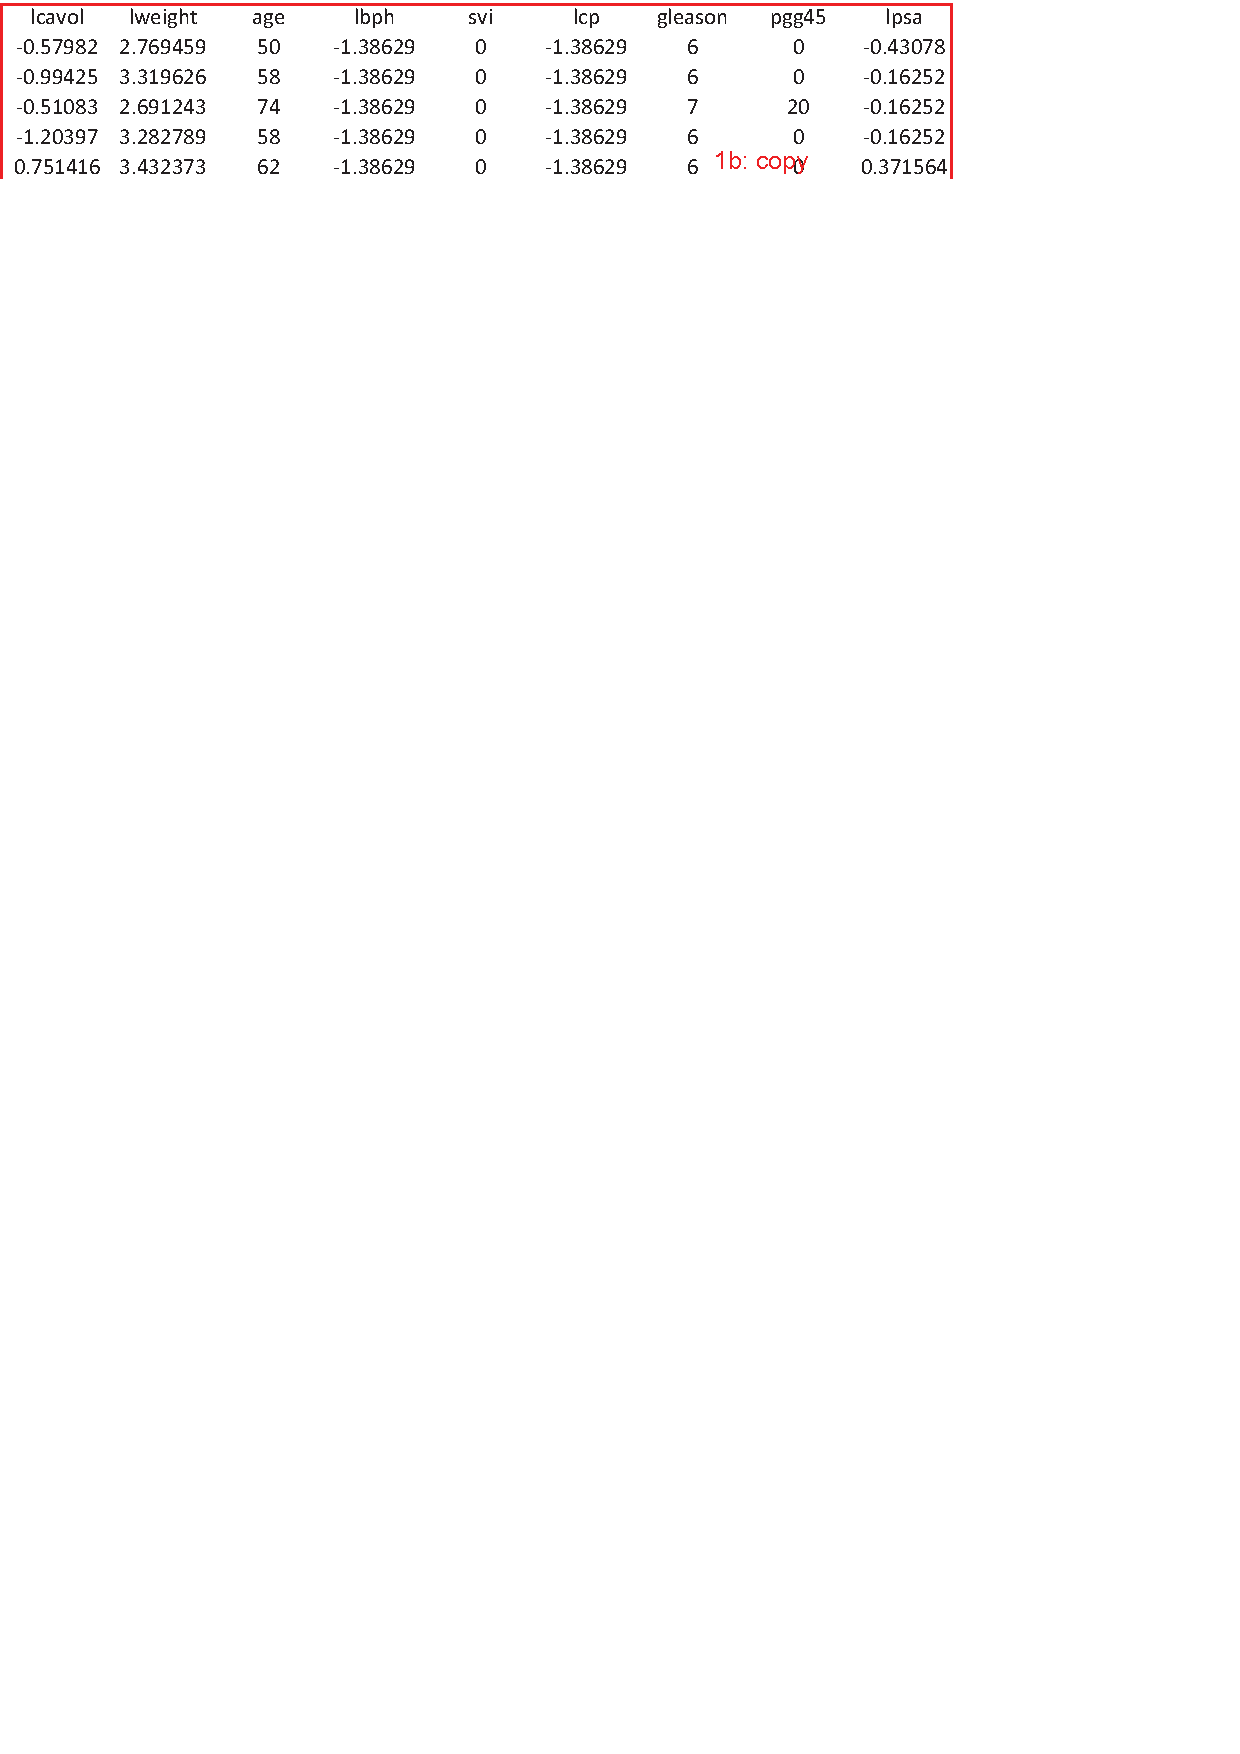
\includegraphics[width=\linewidth, keepaspectratio=true]{img/DataSheet_Prostate_body_markup}
          	\textbf{On the \shtPivot sheet:}
          	\vspace{-20pt}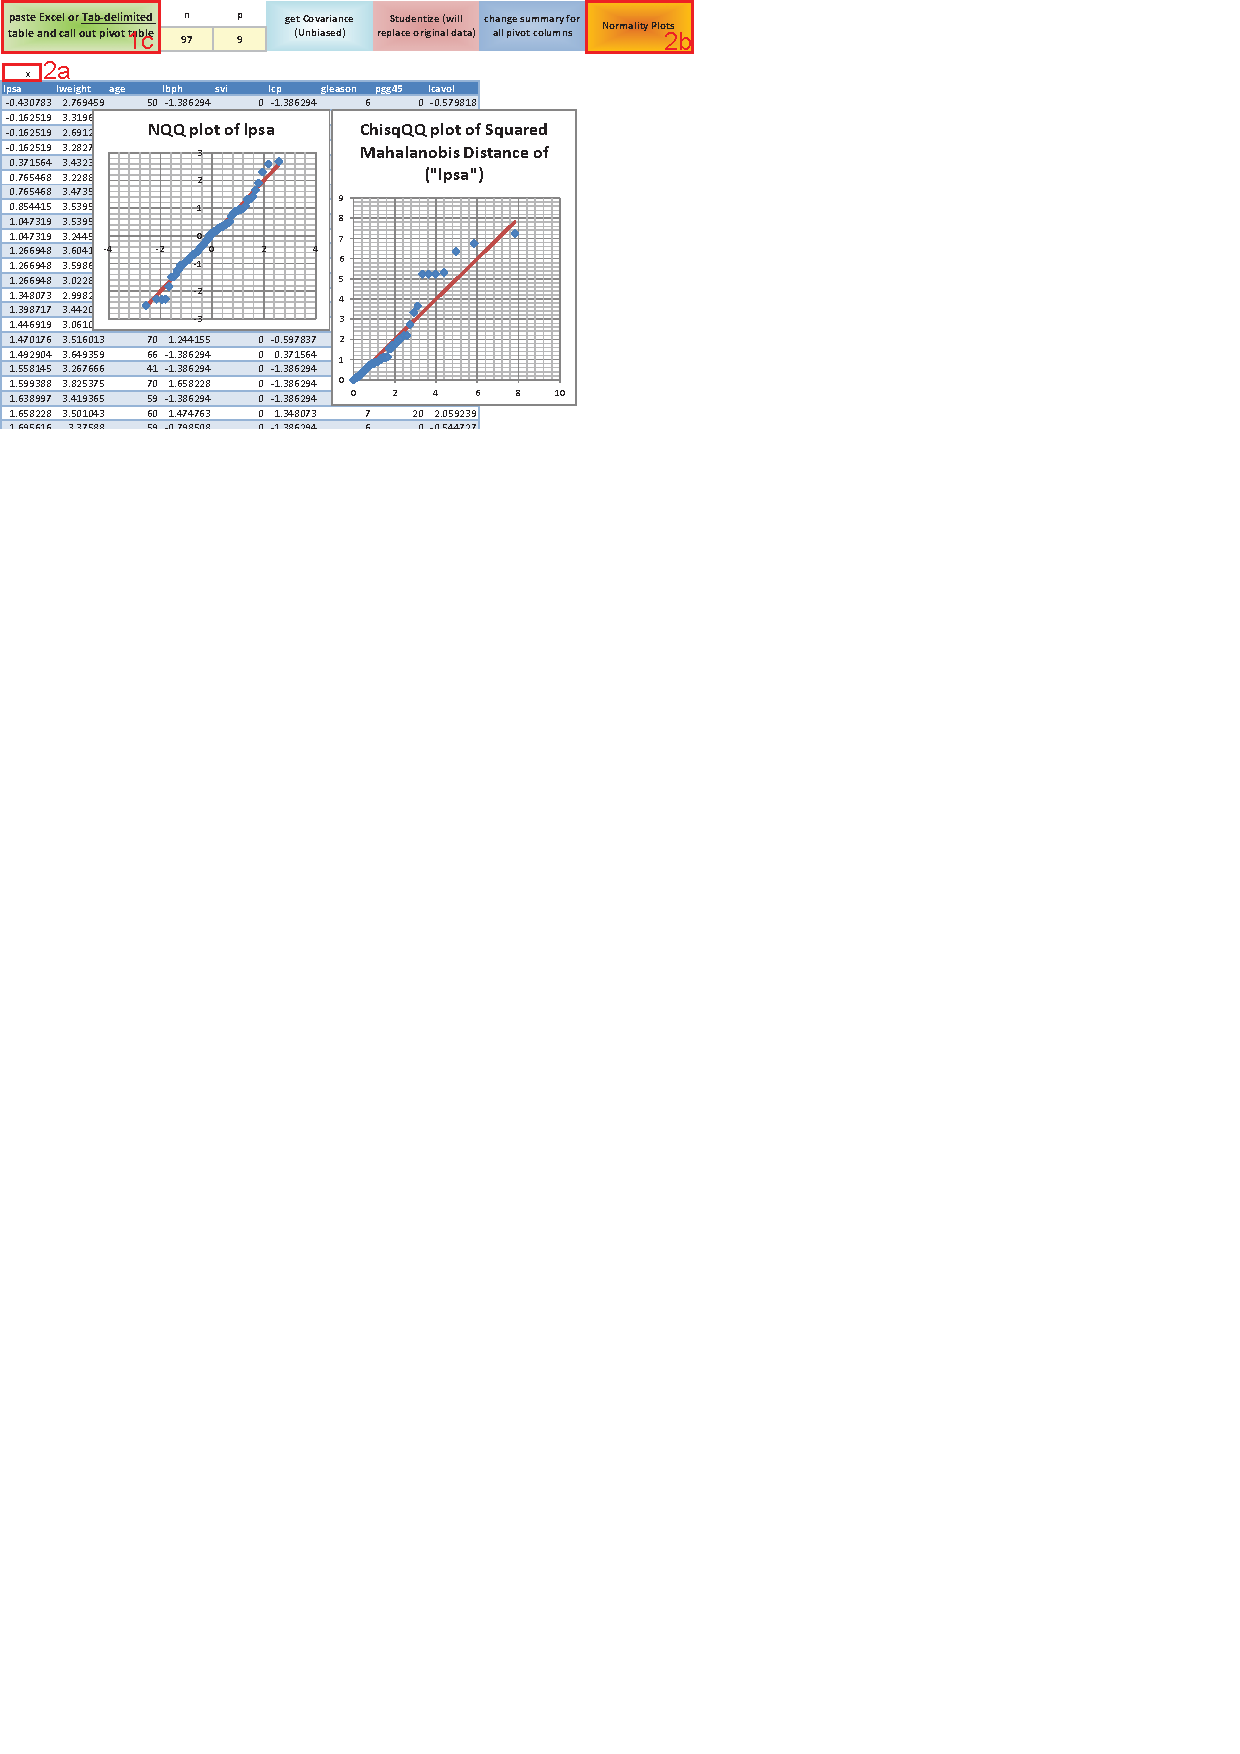
\includegraphics[width=\linewidth, keepaspectratio=true]{img/Prostate_normalityPlots_markup}
          	\centering{}\protect\caption{\textbf{On the ``Data" sheet:} The dataset is registered in the dropdown box by name ``Prostate". The numerical marks have corresponding descriptions in the text. \textbf{On the ``Pivot" sheet:} Some initial exploration in this dataset can be made, for example, starting with normality checks.}\label{fig:DataSheet_Prostate}
          \end{figure}
          \item Select column ``lpsy" by putting an ``x" above the header (a reordering of columns will be triggered to prioritize the selected) and double-click the orange button ``Normality Plots" (
\includegraphics[height=8pt, keepaspectratio=true]{PivotNormalityPlotButton_png}) to have a visual check of the response variable's normality condition. The plots show that the data have a little bit excess kurtosis over that of a normal distribution. Nevertheless, we will proceed for demonstration purpose.
          \item Activate the \shtCorrel sheet. On the \shtCorrel sheet, double-click on the green cell at \texttt{Correl!A26} to copy-paste the dataset from the \shtPivot sheet and augment it with two additional columns: the fitted response ``\texttt{y\_predicted}" and the residuals of fitting. 
          By creating a further copy of the preprocessed data in each analysis sheet, we are free to change the analysis copy without side-affecting other methods on the same preprocessed data.
          \begin{figure}[!tbh]
          	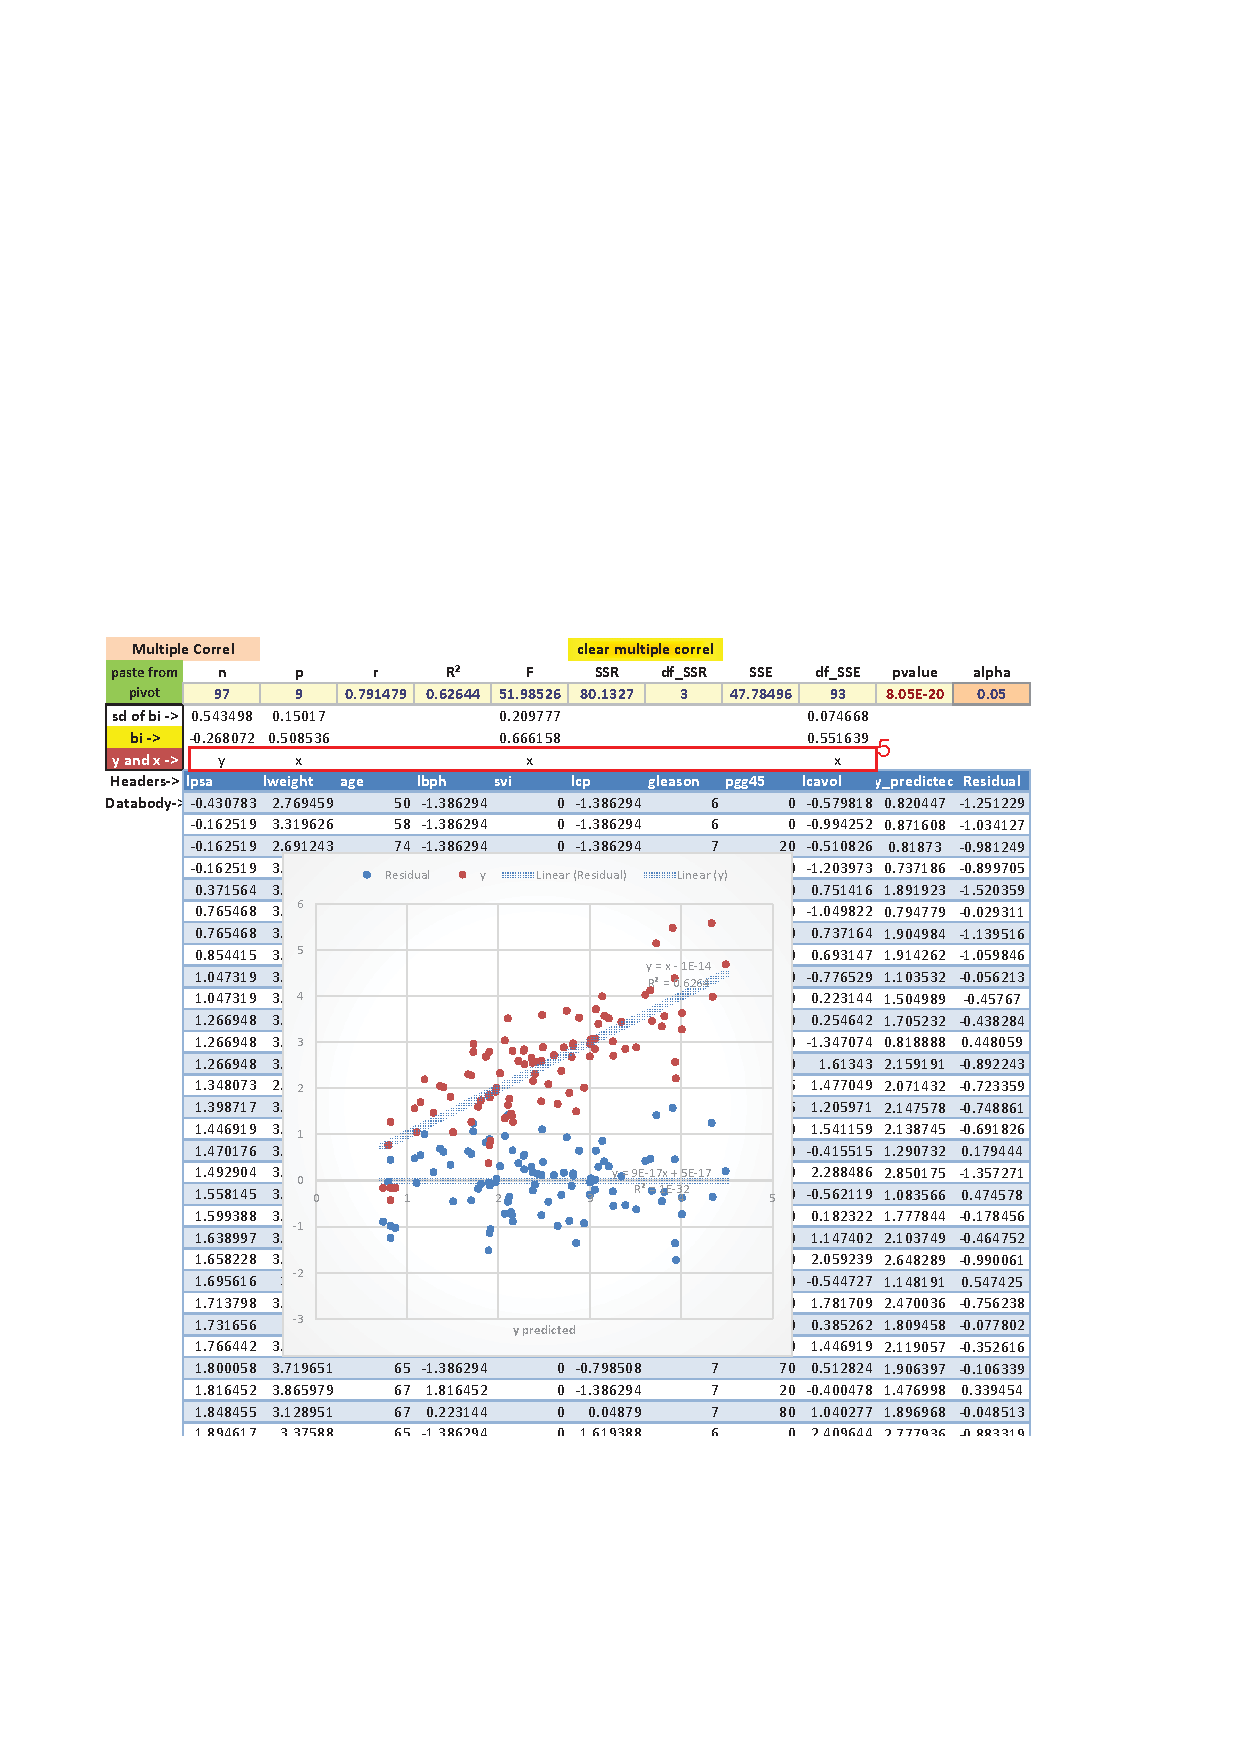
\includegraphics[width=\linewidth, keepaspectratio=true]{img/Correl_multipleRegression_selectedSubset_markup}
          	\vspace{-20pt}\centering{}\protect\caption{Correl sheet: Multiple Regression}\label{fig:Correl sheet: Multiple Regression}
          \end{figure}          
          
          \item Enter ``y" in cell \texttt{Correl!B30} and ``x" to any subset of cells \texttt{Correl!C30:J30} while mointoring the $R^2$ at cell \texttt{Correl!E27}. After a few trials, one may quickly settle to the subset of {``lweight", ``svi", ``lcavol"} giving an $R^2=0.62644$. The implementation hides the trigger of the regression computation in the cell value change event. Whenever the row above the header of the analysis copy of data has some value change, all regression results on the sheet will be refreshed. This allows interactive variable selection to be performed seemlessly. One can then quickly make some visualizations of the numbers. The \shtCorrel sheet now appears as Figure \ref{fig:Correl sheet: Multiple Regression}.
        \end{enumerate}
        One may quickly verify the three ways of computing $R^2$ in multiple regression:
        \[{R^2} = \frac{{SSR}}{{SSR + SSE}} = {\textbf{R}_{yx}}\textbf{R}_{xx}^{ - 1}{\textbf{R}_{xy}} = \textrm{corr}{\left( {y,\hat y} \right)^2}\]
        The second way is coded into the formula for $r$ at cell \texttt{Correl!D27} (Figure \ref{fig:Correl_multipleRegression_Rsquare}). It interprets multiple regression as a process of maximizing the squared correlation between the response and a vector in the linear space spanned by the regressors. And the correlation-maximizing vector is the $\hat y$.
        \begin{figure}[!tbh]
        	\textbf{Multiple Regression $R^2$:}
            \vspace{5pt}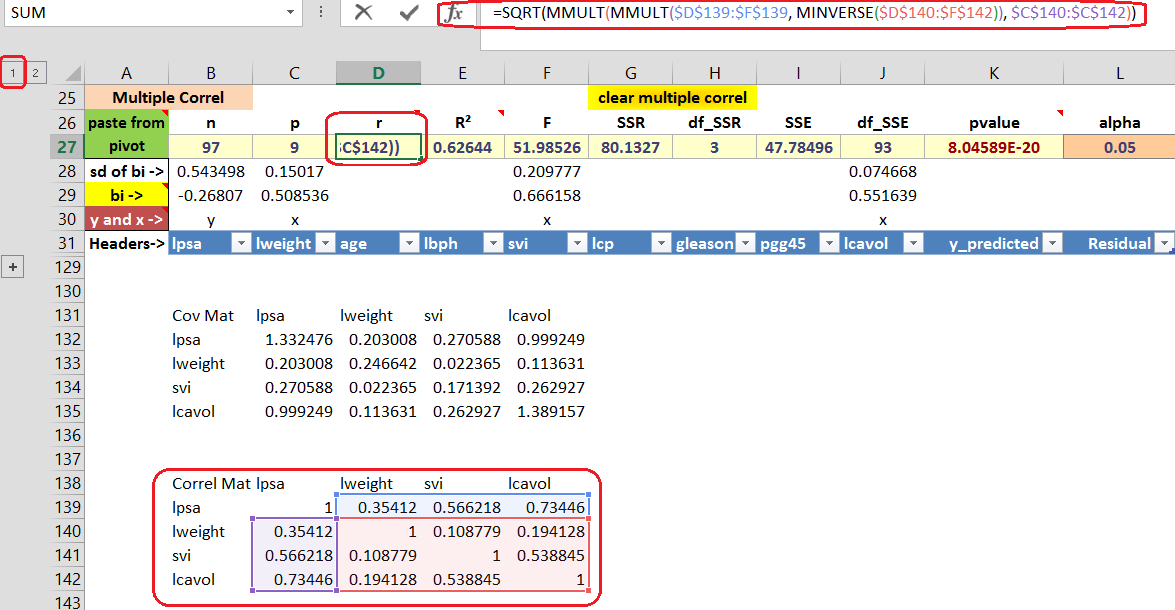
\includegraphics[width=\linewidth, keepaspectratio=true]{Correl_multipleRegression_Rsquare_png}
            \textbf{Testing correlation hypotheses:}
            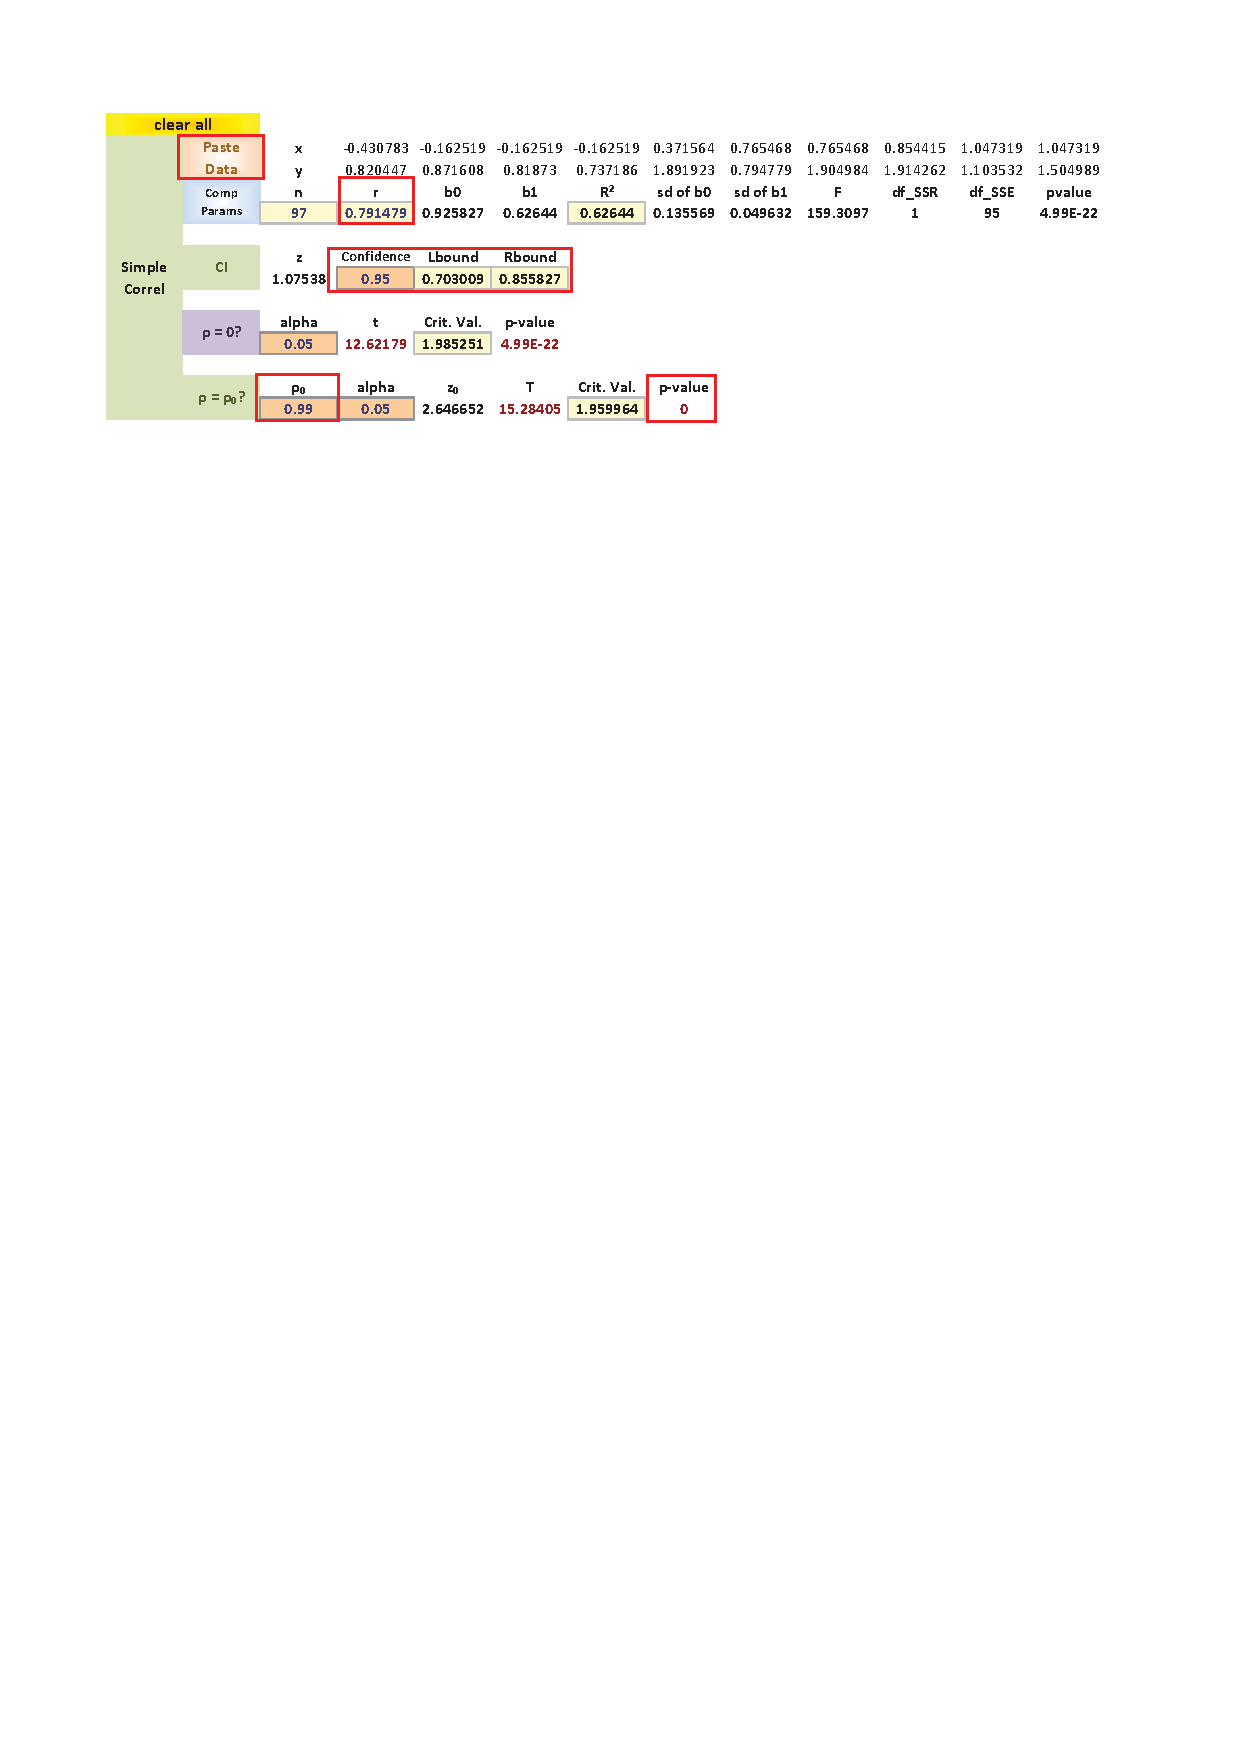
\includegraphics[width=\linewidth, keepaspectratio=true]{img/Correl_simpleCorrel_testing_markup}
            \vspace{-20pt}\centering{}\protect\caption{Multiple Regression $R ^2$ and Hypotheses about Corrlelation}\label{fig:Correl_multipleRegression_Rsquare}
        \end{figure}
        
        Now we test the hypothesis that $R^2$ is close enough to $1$, or, equivalently, $H_0: \textrm{corr} (y, \hat y) = 1$.
        \begin{enumerate}
          \item Select the two columns of ``\texttt{y}" and ``\texttt{y\_predicted}" holding the \texttt{ctrl} key. Copy the selection.
          \item Double click cell \texttt{Correl!B2}. 
          A few results are already shown. For example, the 95\%-confidence interval of $\textrm{corr} (y, \hat y)$ is $[0.703,0.856]$ based on the Fisher $z$-transform \citep{Fisherztransform1915}.
          \item Enter $0.99$ in  cell \texttt{Correl!C14}. The p-value of testing $H_0: \textrm{corr} (y, \hat y) = 0.99$ shows up as 0 in cell \texttt{Correl!H14} indicating the model has left unexplained a non-zero portion of variability in the response variable.
        \end{enumerate}
        
        \subsection[egLM]{Multivariate Regression Involving Categorical Variables}
        In a general regression setup, one frequently encounters more than one response variable and categorical variables in the regressors. The \shtLM sheet is implemented for this task. LM stands for Linear Model. The initiation step is similar as before: after the data is pasted to the \shtPivot sheet and preprocessed there, one switch to the \shtLM sheet and double-clicks the green paste-from-pivot button at the top-left corner to create a working copy of the dataset. One then specifies a \texttt{y} ahead of each response column, an \texttt{x} ahead of each continuous regressor column and a \texttt{c} ahead of each categorical regressor column. A second specification, regarding Rectangle 3 of Figure \ref{fig:LMSheetOutput_markup}, is needed to indicate which of the \texttt{x} and \texttt{c} columns will finally be used with an \texttt{x} in the cells above the Working Data. Note that the categorical variables in Rectangle 2 are auto-encoded into dummy variables of Rectangle 4 in Figure \ref{fig:LMSheetOutput_markup}. The coefficient and standard deviation estimates the multivariate regression are output in Rectangle 6.
        In addition to estimation of the regression coefficients, the sheet also implements Multivariate-ANOVA tests, a SAS \texttt{proc glm} code generator macro, and transformation matrices on both continuous responses and continuous regressors.
        \begin{figure}[!tbh]
                \centering
                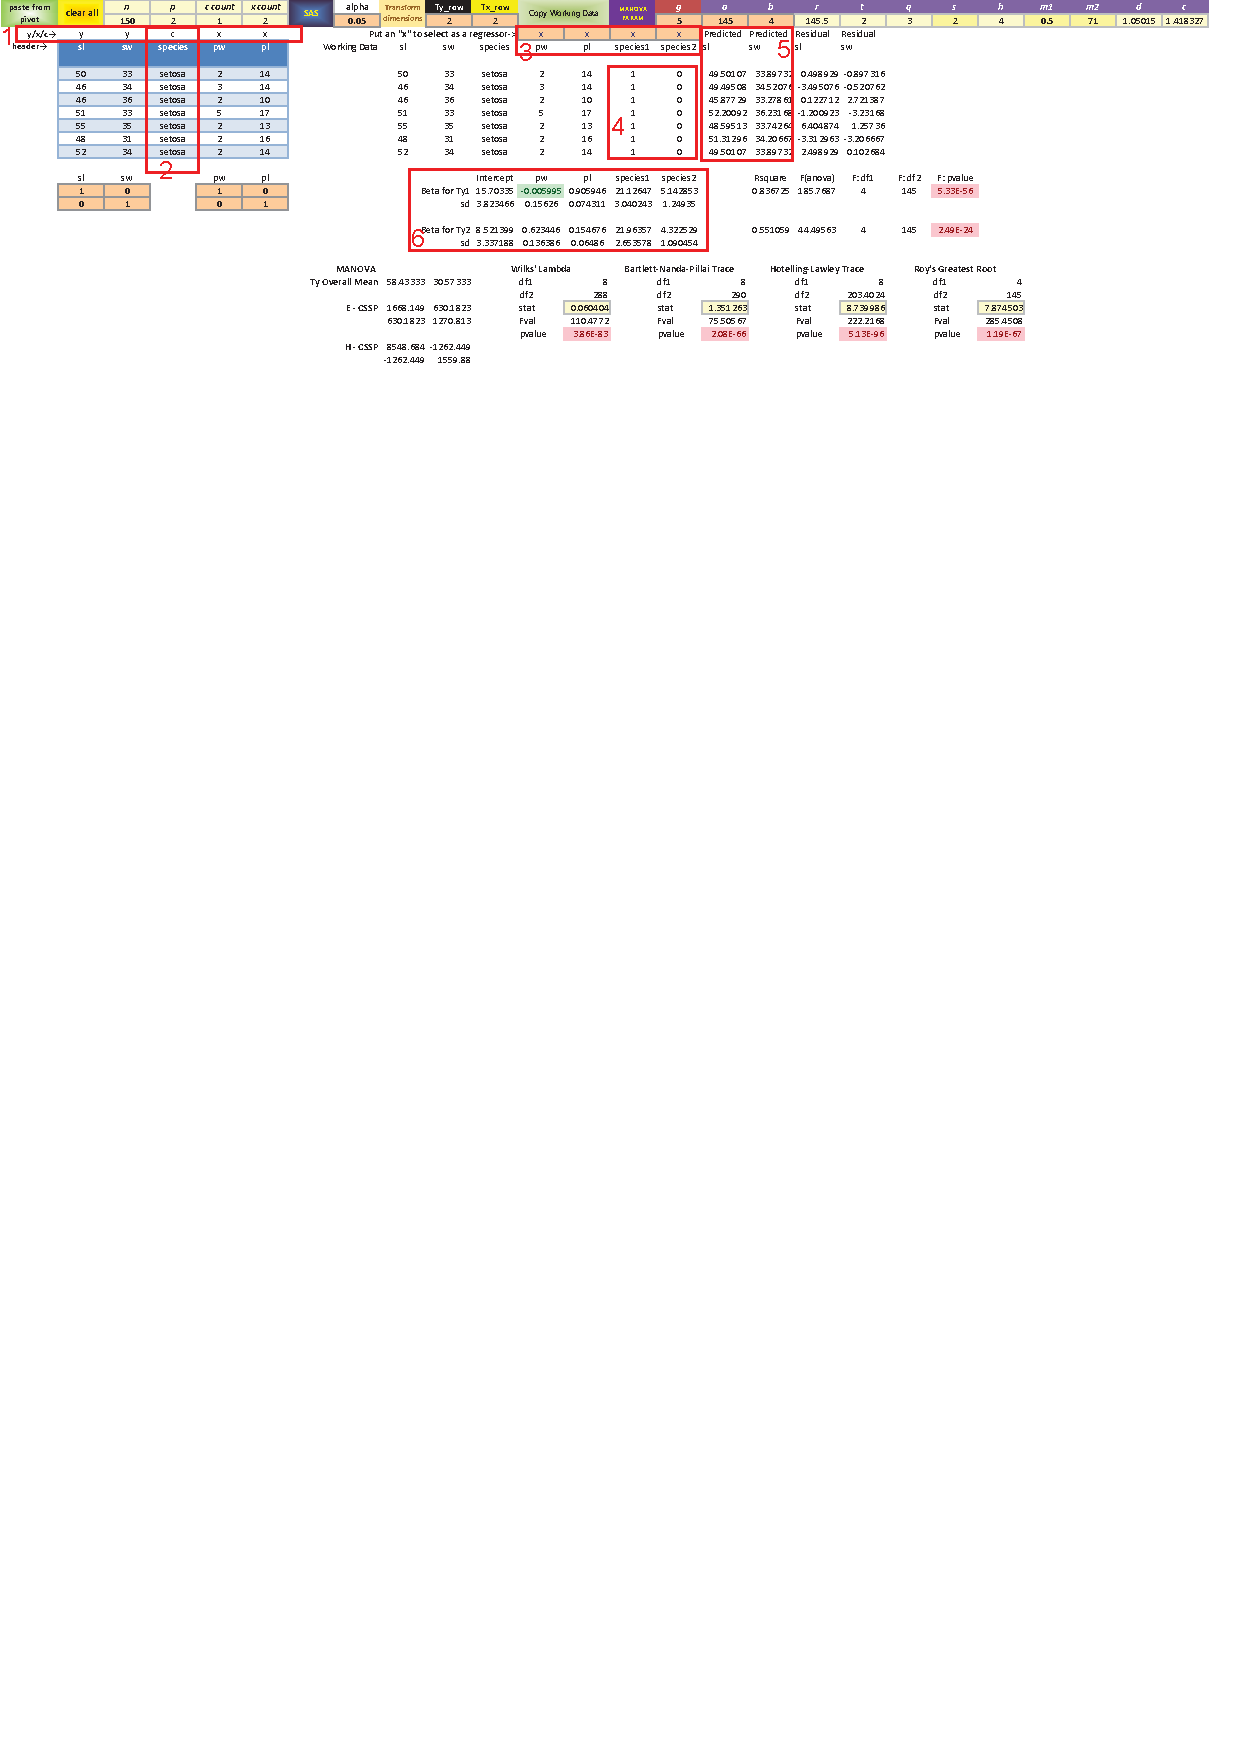
\includegraphics[width=\linewidth, keepaspectratio=true]{img/LMSheetOutput_markup}
                \vspace{-20pt}\centering{}\protect\caption{Output of the Linear Model sheet}\label{fig:LMSheetOutput_markup}
        \end{figure}
        
        \subsection[egOneSample]{Multivariate Hypothesis Testing with Excel Tool}
        
        
        Many hypotheses about the differences of \emph{correlated} variables can be tested using Hotelling's $T^2$ statistic. The $T^2$ statistic is a multivariate generalization of Student's $t$ statistic. It takes a quadratic form and its sampling distribution is linked to the $F$-distribution \citep{hotelling1931Tsq}:
        
        \[n{\left( {\bar{\textbf{x}} - {\boldsymbol{\mu}}} \right)^ \intercal}{\textbf{S}^{ - 1}}\left( {\bar{\textbf{x}} - {\boldsymbol{\mu}}} \right) \sim T^2(p, n-1) = \frac{{p\left( {n - 1} \right)}}{{n - p}}F\left( {p,n - p} \right) \]
        
        where $\textbf{x} \in \mathbb{R}^{p\times n}$ is the data vector, 
        $\bar{\textbf{x}} \in \mathbb{R}^p$ is the sample mean vector, 
        $\boldsymbol{\mu} \in \mathbb{R}^p$ is the true mean vector,
        $n$ is the sample size, and 
        $\textbf{S}$ is the sample covariance matrix
        \[\textbf{S} = \frac{1}{{n - 1}}\left( {\textbf{x} - \bar{\textbf{x}}{\textbf{1}^\intercal}} \right){\left( {\textbf{x} - \bar{\textbf{x}}{\textbf{1}^\intercal}} \right)^\intercal}.\]
        
        
        If the sample covariance $\textbf{S}$ is replaced by the true covariance
        $\boldsymbol{\Sigma}$ then the resulting pivotal quantity $n{\left( {\bar{\textbf{x}} - {\boldsymbol{\mu}}} \right)^ \intercal}{\boldsymbol{\Sigma}^{ - 1}}\left( {\bar{\textbf{x}} - {\boldsymbol{\mu}}} \right)$
        is $\chi^2$-distributed.
        Since any linear transformation of a normal random vector remains normal, the test statistic remains $T^2$. One then focuses on the design of a linear transform $C$ that represents the hypothesis of interest: 
        
        \[H_0: C\bar{\textbf{x}} - \boldsymbol{\xi}_0 = \textbf{0}.\]
        
        
        
        Since the design of the linear transform is essentially a process of choosing the proper basis for a re-coordinatization of data, the whole process can be intuitively understood as finding the most direct ``angle" to view the data such that the hypothesis is settled by judging whether the distance between a pair of points is too much for them to be considered the same point. We demonstrate the methodology using the classic example of \cite{rao1948corkboring} with our Excel tool.
        
        
        
        \subsubsection{Example: Bark deposit from 4 directions of the trunk of 28 Oak trees.}
        
        \cite{rao1948corkboring} exhibited a dataset containing measurements of the weights of  cork borings taken from 4 directions on the trunk of 28 Oak trees. The hypothesis of interest was that the deposit is uniform in the North--South directions and also uniform but \emph{less} in the East--West directions. The dataset is registered under name "Cork borings" on the \shtData sheet. As before, a copy is pasted to the \shtPivot sheet for any preprocessing and initial exploration. Then a further copy for analysis is pasted to the \shtTsquare sheet by double-clicking the green paste button placed at the top-left cornor of each sheet. The initial setup should appear as Figure \ref{fig:corkboringinitialsetup}.
        \begin{figure}[!tbh]      
        	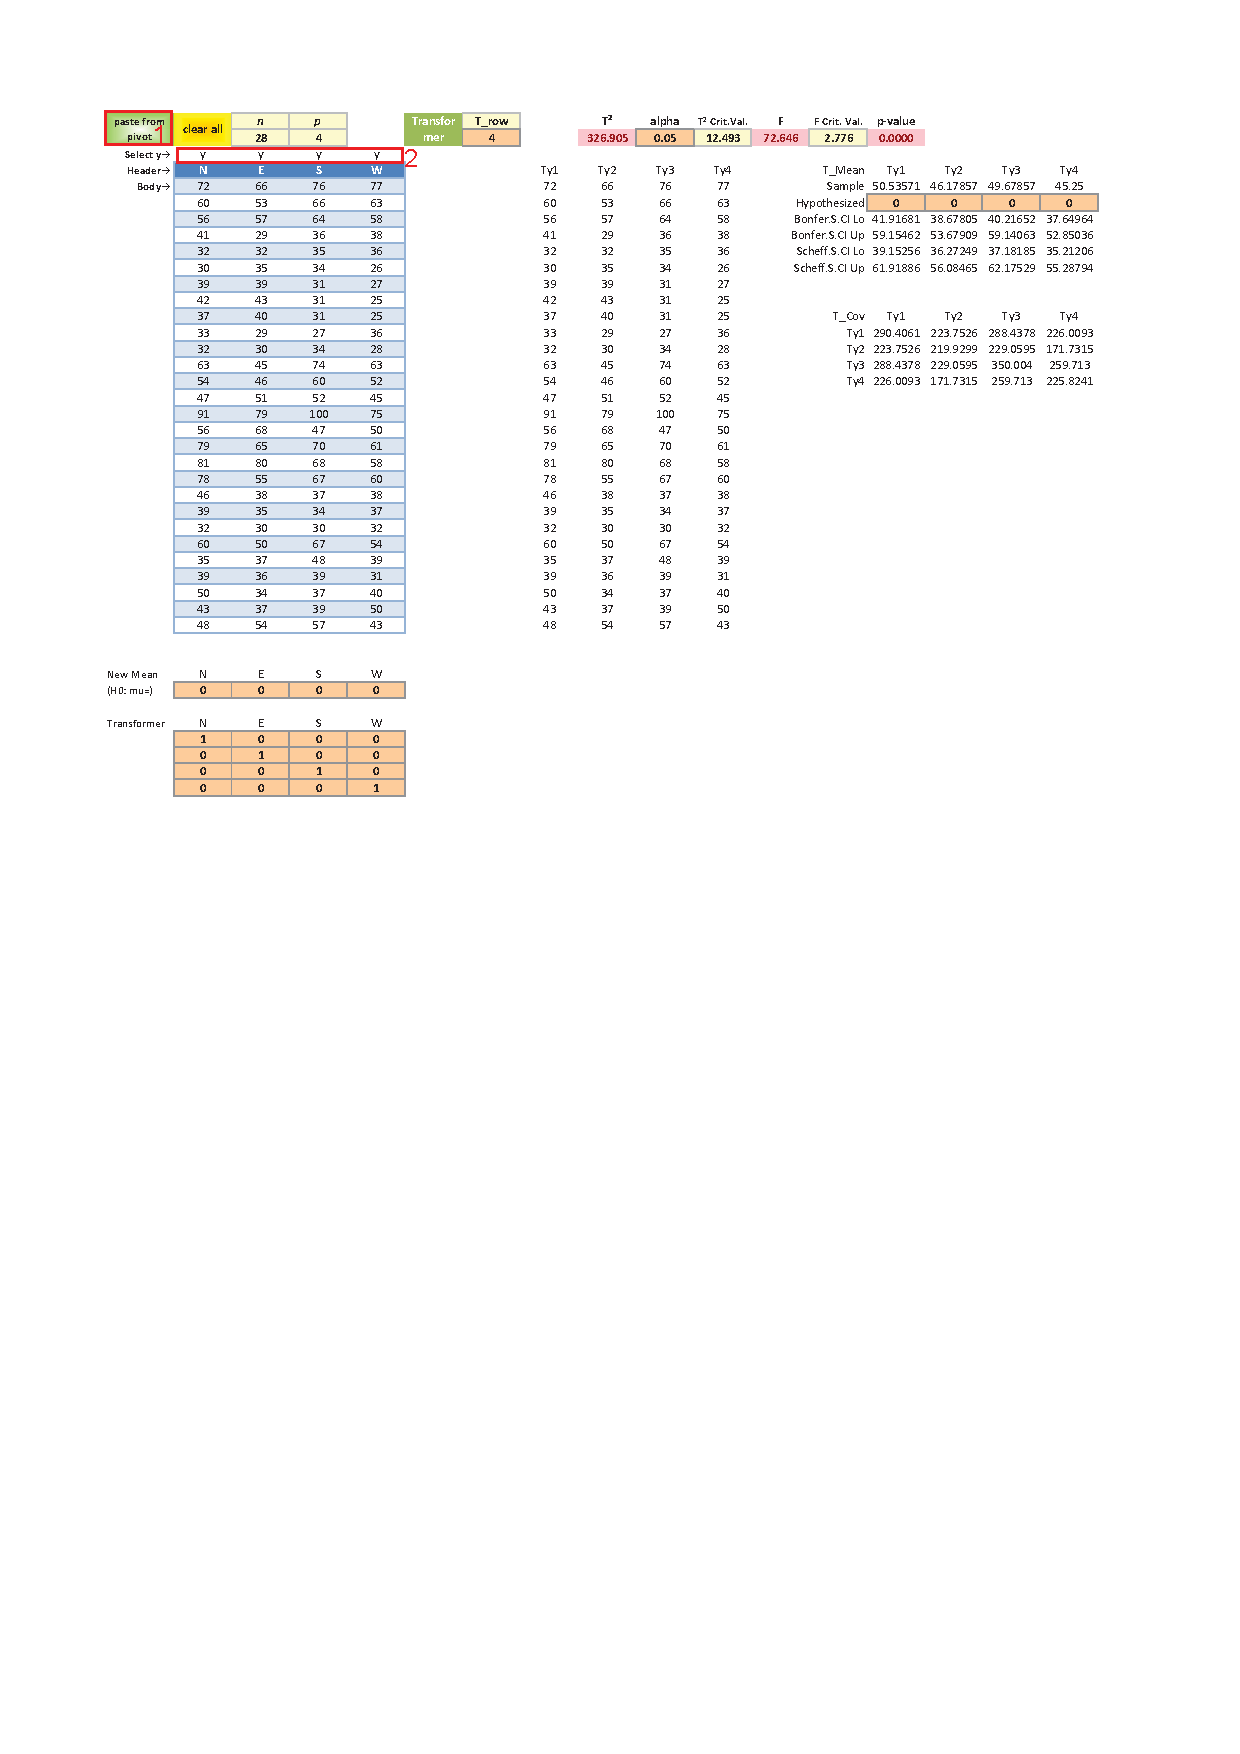
\includegraphics[width=\linewidth, keepaspectratio=true]{img/TsquareSheetAfterPaste_markup}
        	\vspace{-25pt}\centering{}\protect\caption{Tsquare sheet: initial setup.}\label{fig:corkboringinitialsetup}
        \end{figure}
        
        \begin{enumerate}
                
                
                
                \item Perform the following three steps exactly: Select cells \texttt{Tsquare!B3:E3} | press \texttt{y} on the keyboard | Windows user: press \texttt{ctrl} + \texttt{Enter} on the keyboard; Mac user: Press \texttt{command} + \texttt{Enter}. By doing these steps, you have entered 4 ``y"s simultaneously.
                
                
                
                Now the data has been loaded onto the \shtTsquare sheet, we proceed to test some hypotheses. We start with the univariate null hypothesis $H_0: N = S$. The following step show the p-value of this test in \texttt{Tsquare!N2}, which is 0.5740 and the null hypothesis therefore accepted.
                \item Enter $-1$ in cell \texttt{Tsquare!D39} such that the first row of the matrix of our linear transform becomes $(1,0,-1,0)$. Enter 1 in cell \texttt{Tsquare!G2} to indicate we use only the first row of the transformation matrix. The \shtTsquare sheet should now appear as
                
                \begin{figure}[!tbh]
                        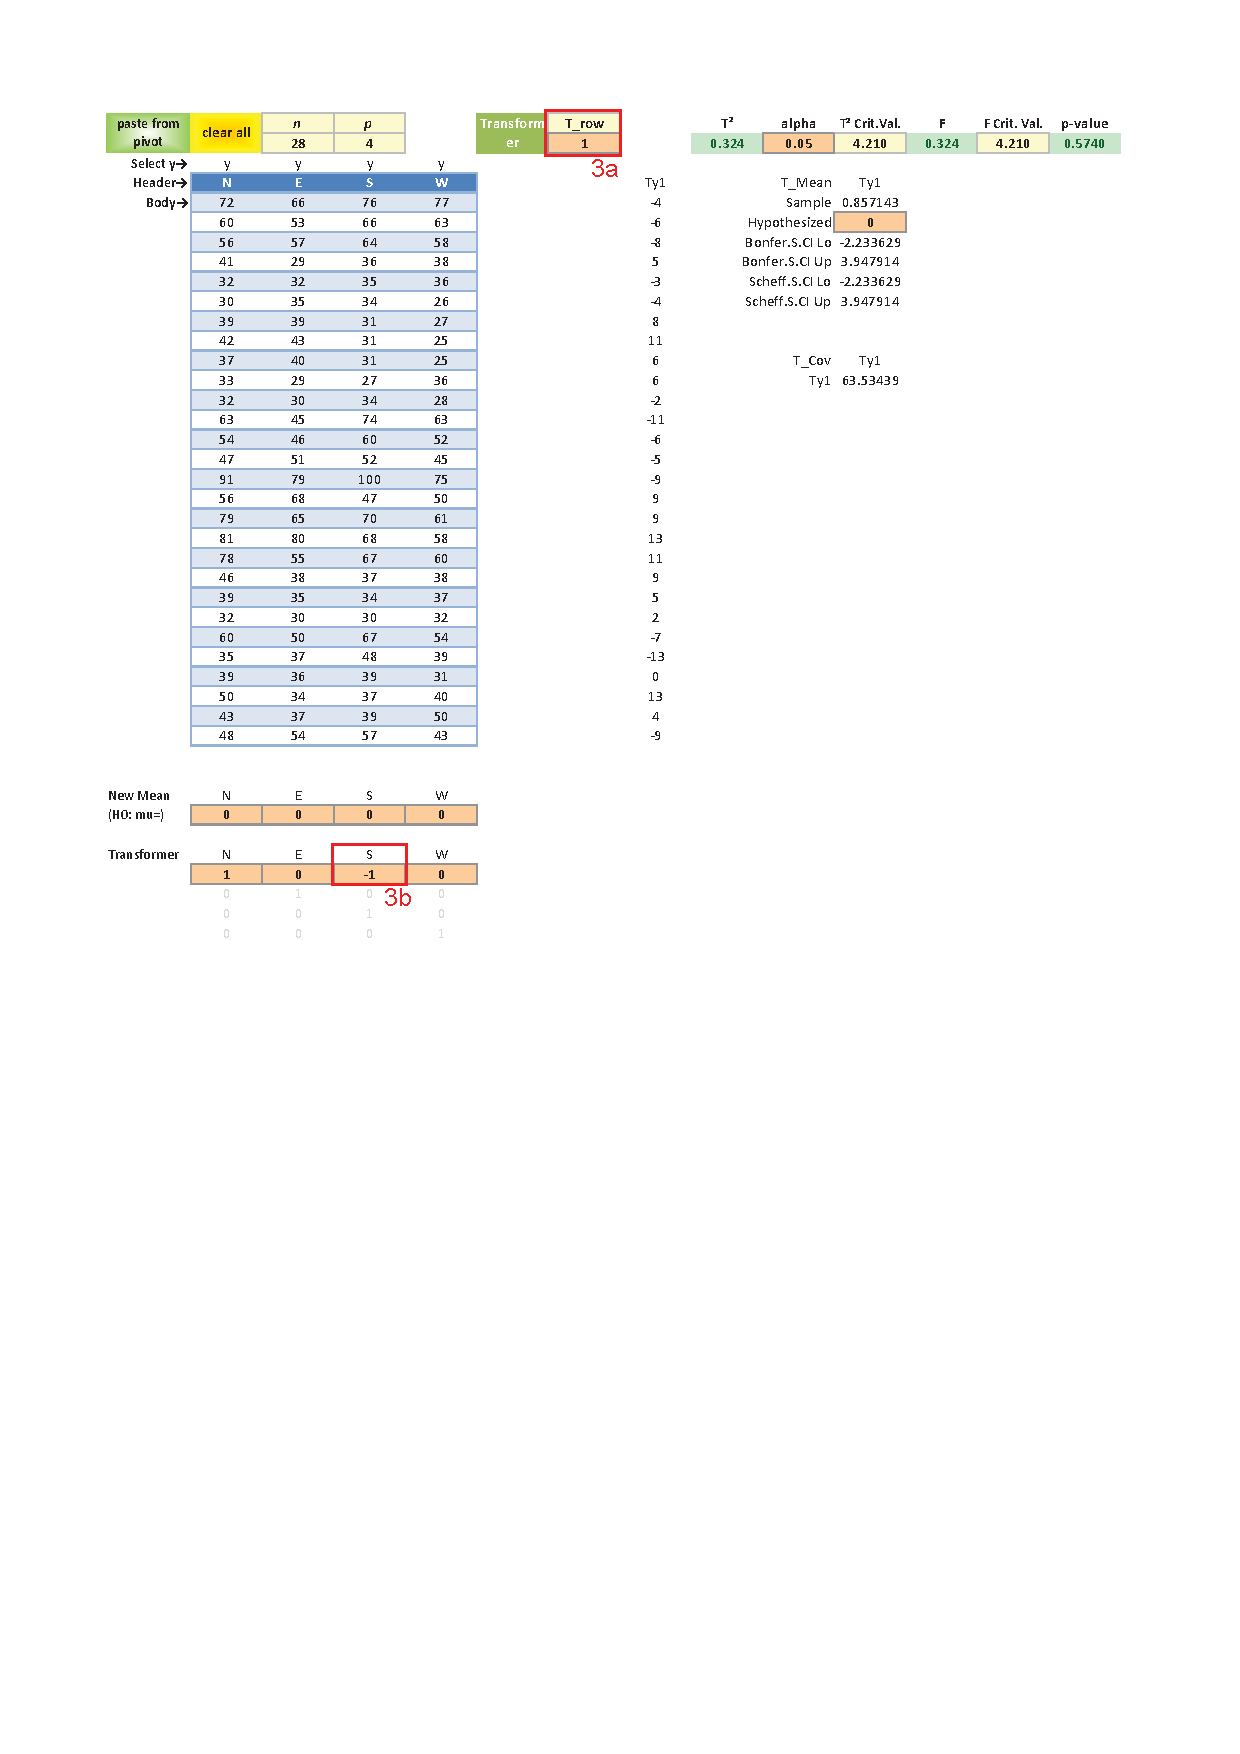
\includegraphics[width=\linewidth,keepaspectratio=true]{img/TsquareSheetOutput_markup}
                        \vspace{-25pt}\centering\protect\caption{Tsquare sheet: Testing $H_0: N = S$}
                \end{figure}
                
                
                
                Next we test the another univariate hypothesis $H_0: E = W$. The following step results in a p-value=0.6310 and therefore the null hypothesis is accepted.
                
                \item Modify the first row of the transformation matrix near \texttt{Tsquare!B39:E39} into $(0,1,0,-1)$. The \shtTsquare sheet should now appear as
                \begin{figure}[!tbh]
                        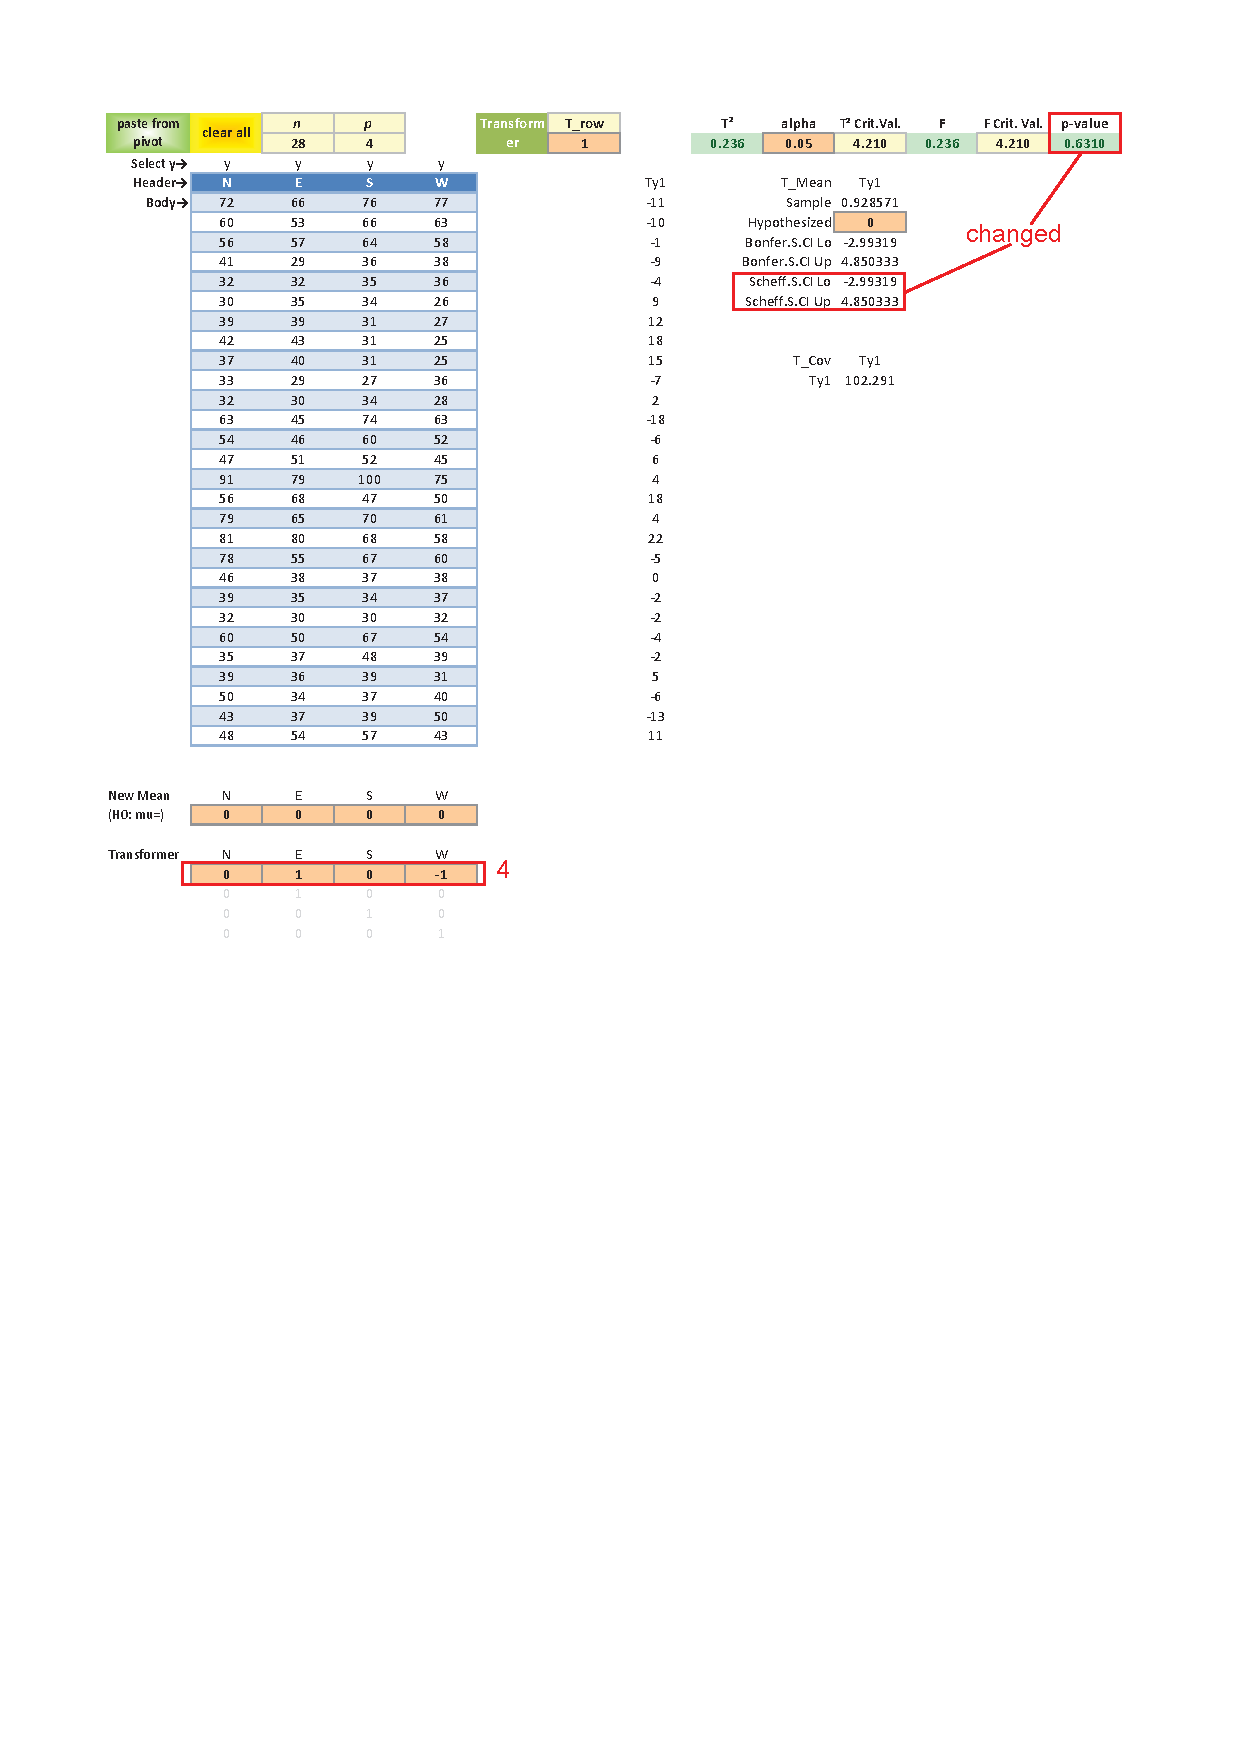
\includegraphics[width=\linewidth,keepaspectratio=true]{img/TsquareSheetOutput2_markup}
                        \vspace{-25pt}\centering\protect\caption{Tsquare sheet: Testing $H_0: E = W$}
                \end{figure}
                
                
                Next we test the two hypotheses jointly: $H_0: N=S$ and $E=W$. The following step results in an increased p-value=0.8194 and therefore null hypothesis accepted.
                
                \item Change \texttt{Tsquare!G2} to 2 and modify the first 2 rows of the transformation matrix near \texttt{Tsquare!B39:E40} into 
                \[\left[ {\begin{array}{*{20}{c}}
                        1&0&-1&0 \\ 
                        0&1&0&-1
                        \end{array}} \right]\]
                
                
                The \shtTsquare sheet should now appear as
                \begin{figure}[!tbh]
                        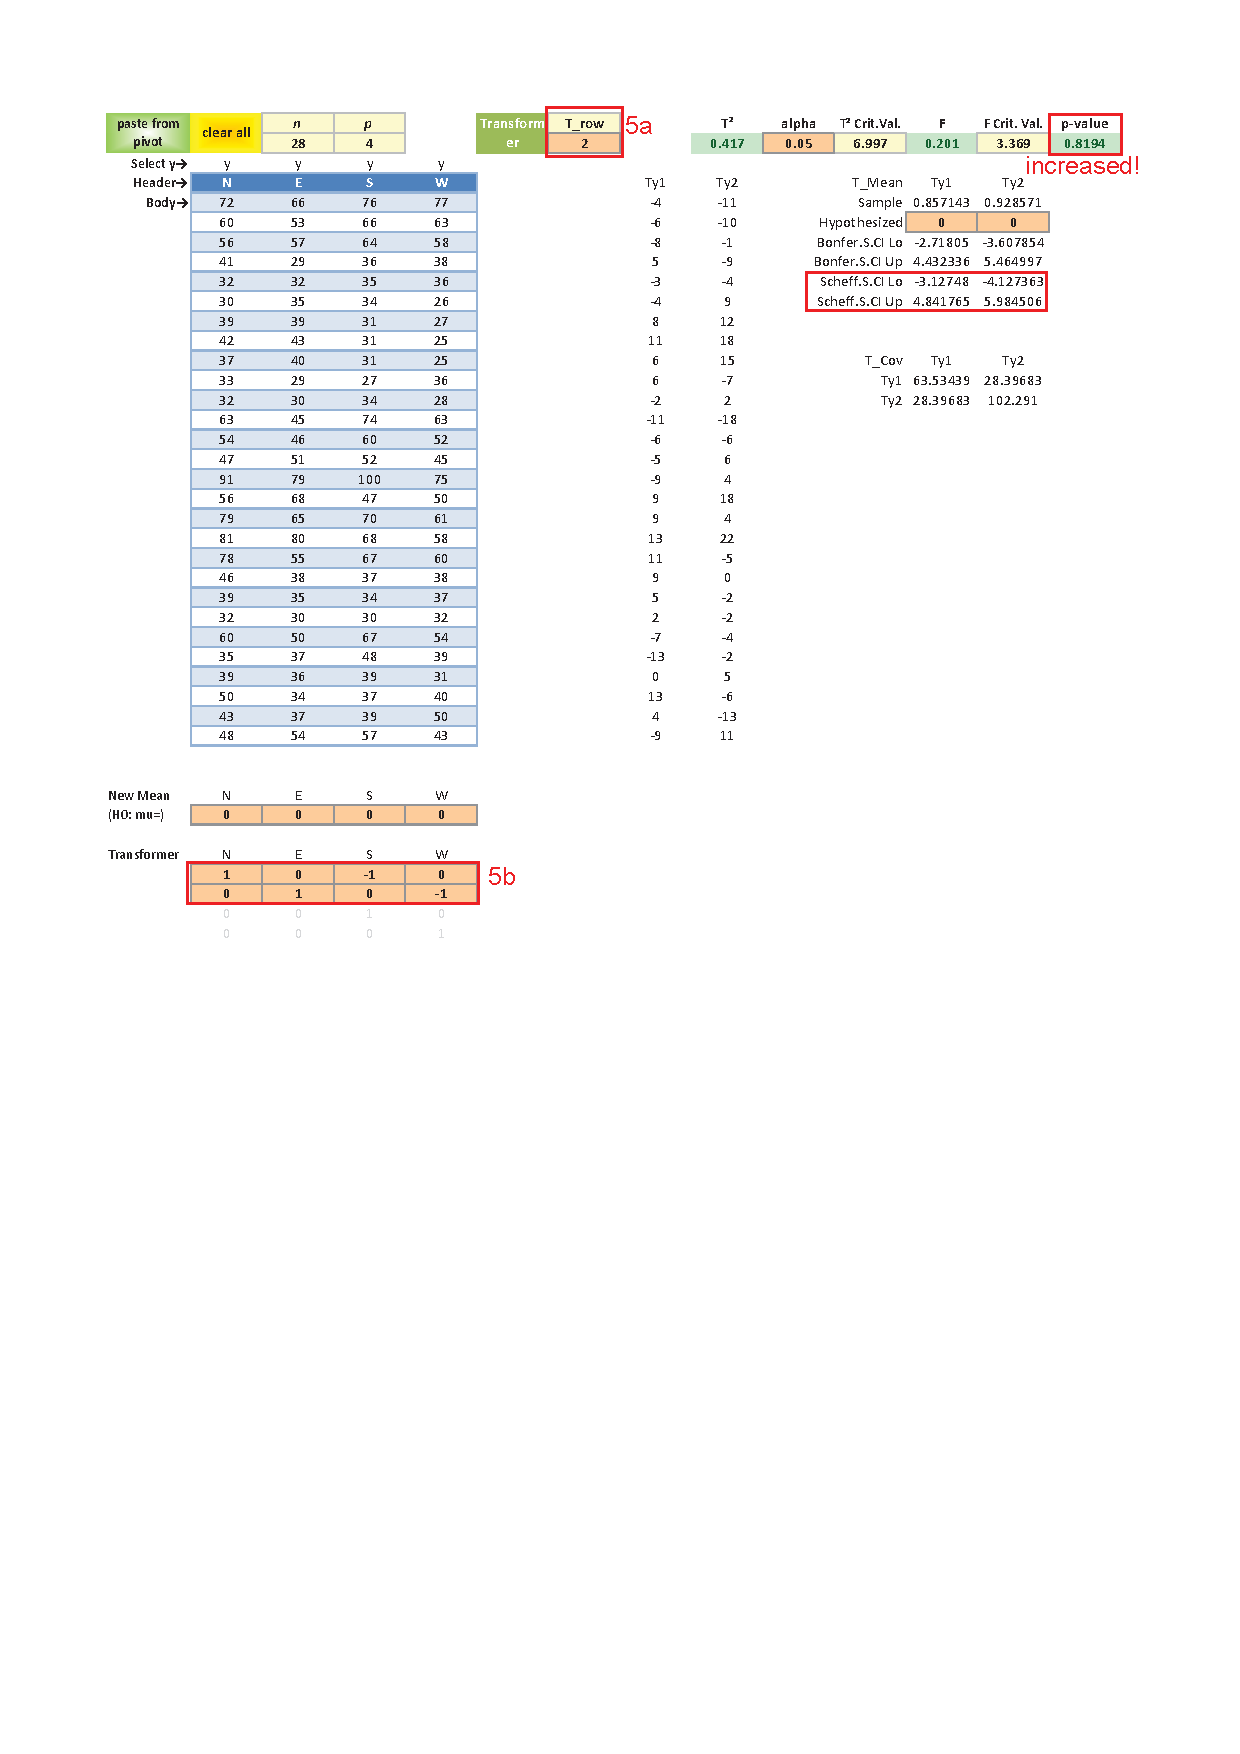
\includegraphics[width=\linewidth,keepaspectratio=true]{img/TsquareSheetOutput3_markup}
                        \vspace{-20pt}\centering\protect\caption{Tsquare sheet: Testing $H_0: N = S \texttt{ and } E=W$}
                \end{figure}
                
                \item To understand why the p-value has increased in the previous step, we plot the covariance matrix of the transformed data. Now perform the following steps: copy \texttt{L14:M15}, the covariance of the transformed data (\texttt{Ty1, Ty2}), switch to the \shtCovCorrel sheet, double-click on the wide green cell \texttt{Cov2Correl!A3}, double-click on the orange cell \texttt{Cov2Correl!Q1}, follow the instruction on the popup to pick the covariance range at \texttt{Cov2Correl!B4:C5} and click done. Figure \ref{fig:Cov2Correl_PlotCov} should appear on the \shtCovCorrel sheet now.
                
                \begin{figure}
                        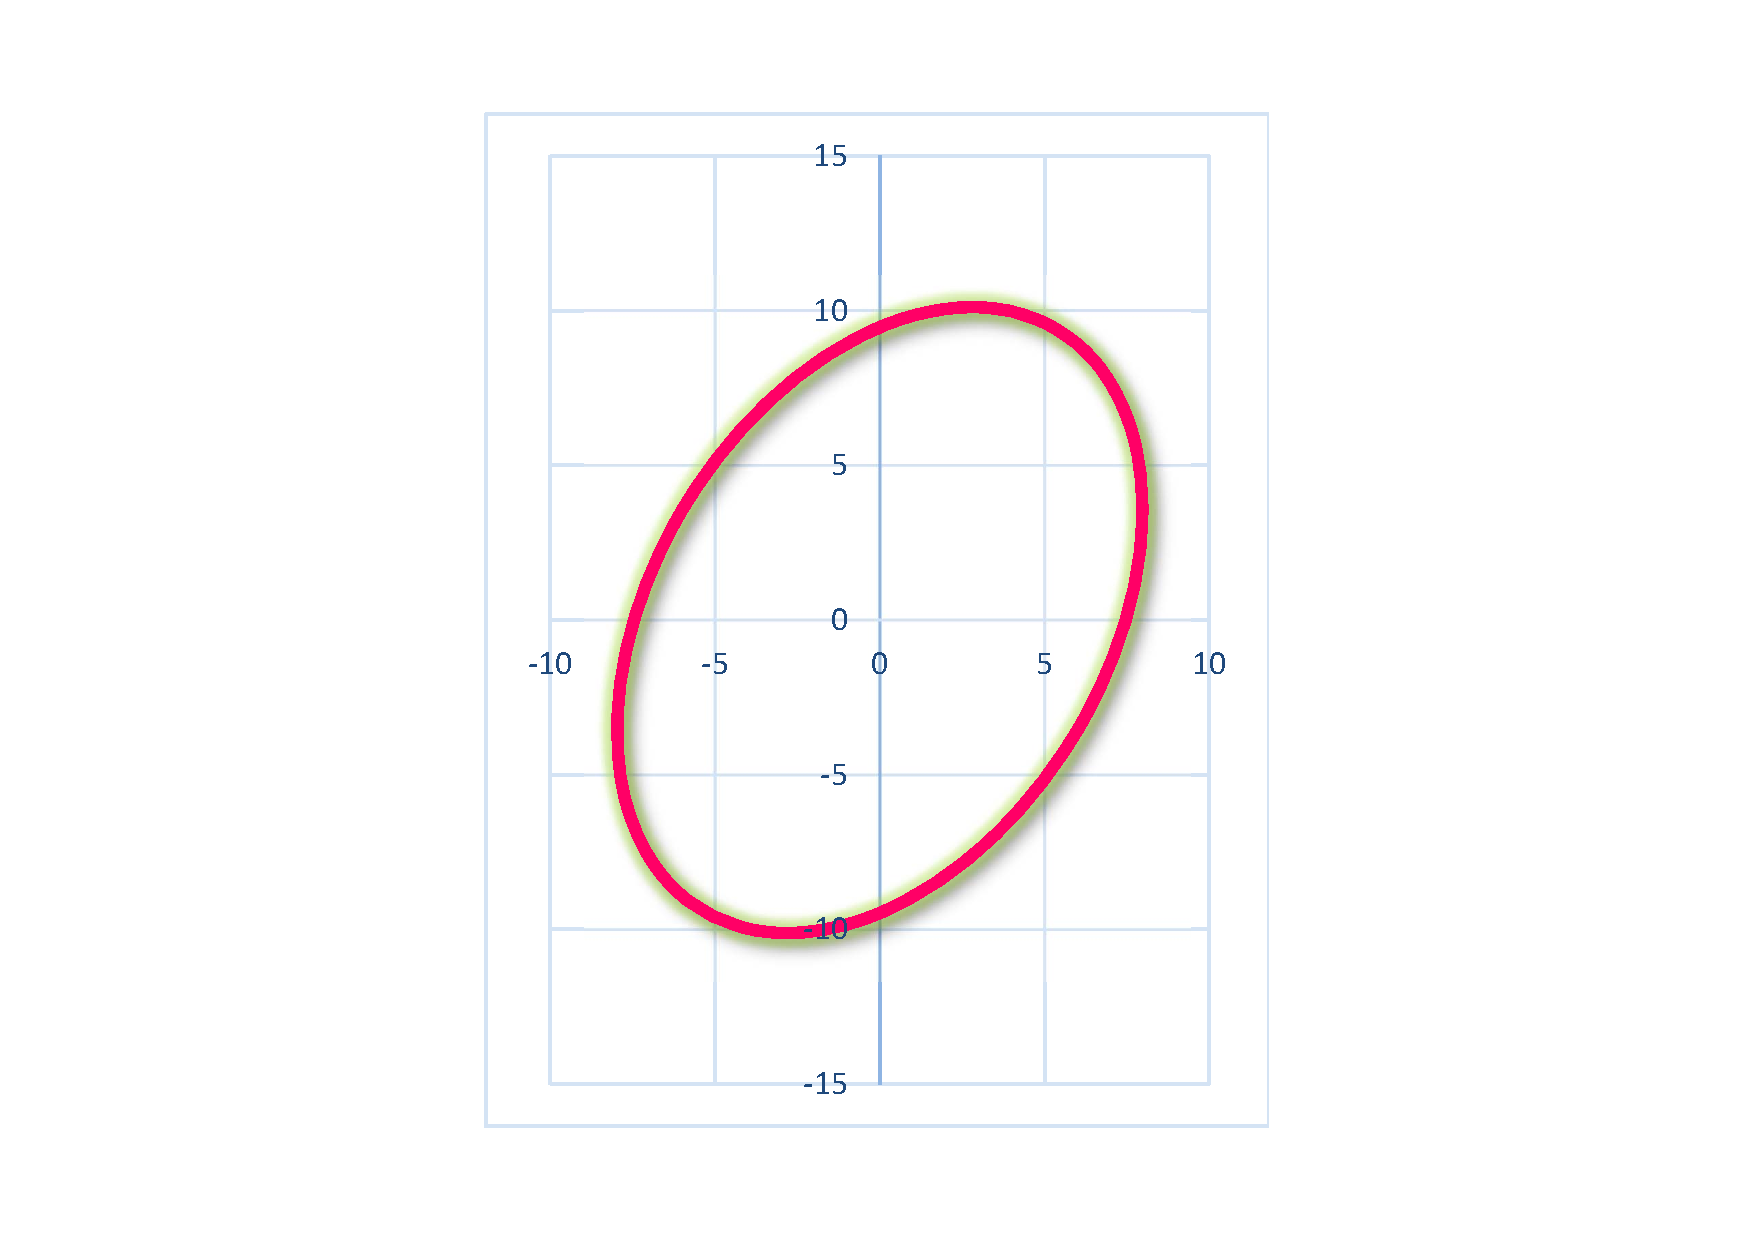
\includegraphics[width=130pt,keepaspectratio=true]{img/Cov2Correl_PlotCov}
                        \vspace{-20pt}\centering\protect\caption{Cov2Correl sheet: Covariance plot of the transformed responses.}\label{fig:Cov2Correl_PlotCov}
                \end{figure}
                
        \end{enumerate}
        
        Now we see that the covariance is elongated along the positive sloped direction, making it possible that the mean vector (\texttt{0.857142857, 0.928571429}), displayed at range \texttt{Tsquare!L5:L6}, has a smaller Mahalanobis distance from the center than both its projections on the two standard basis coordinates. This should be understood in common-sense language that the two hypotheses corroborate each other. The data has indicated that it is more natural to have $N=S$ and $E=W$ happening together than separately, and it is rather strange to observe uniformity in only one of the directions but not in the other. The corroboration effect would not have been captured had we been testing only univariate procedures.
        
        
        To test that the $E-W$ direction is less uniform than the $N-S$ direction, we use the linear combination $(N-S)-(E-W)$ and the null hypothesis that the two directions are equally uniform so that linear combination has zero mean under the null. On the \shtTsquare sheet, we change back to use only the 1st row of the transform matrix by setting \texttt{Tsquare!G2} to 1 and enter $(1,-1,-1,1)$ as the 1st row at \texttt{Tsquare!B39:E39}. The test result accepts the null with an even bigger p-value=0.9714 (\texttt{Tsqaure!N2}). Looking into the data, we do find a number of points where the difference between $N-S$ is greater than that between $E-W$.
        
        \begin{figure}[!tbh]
                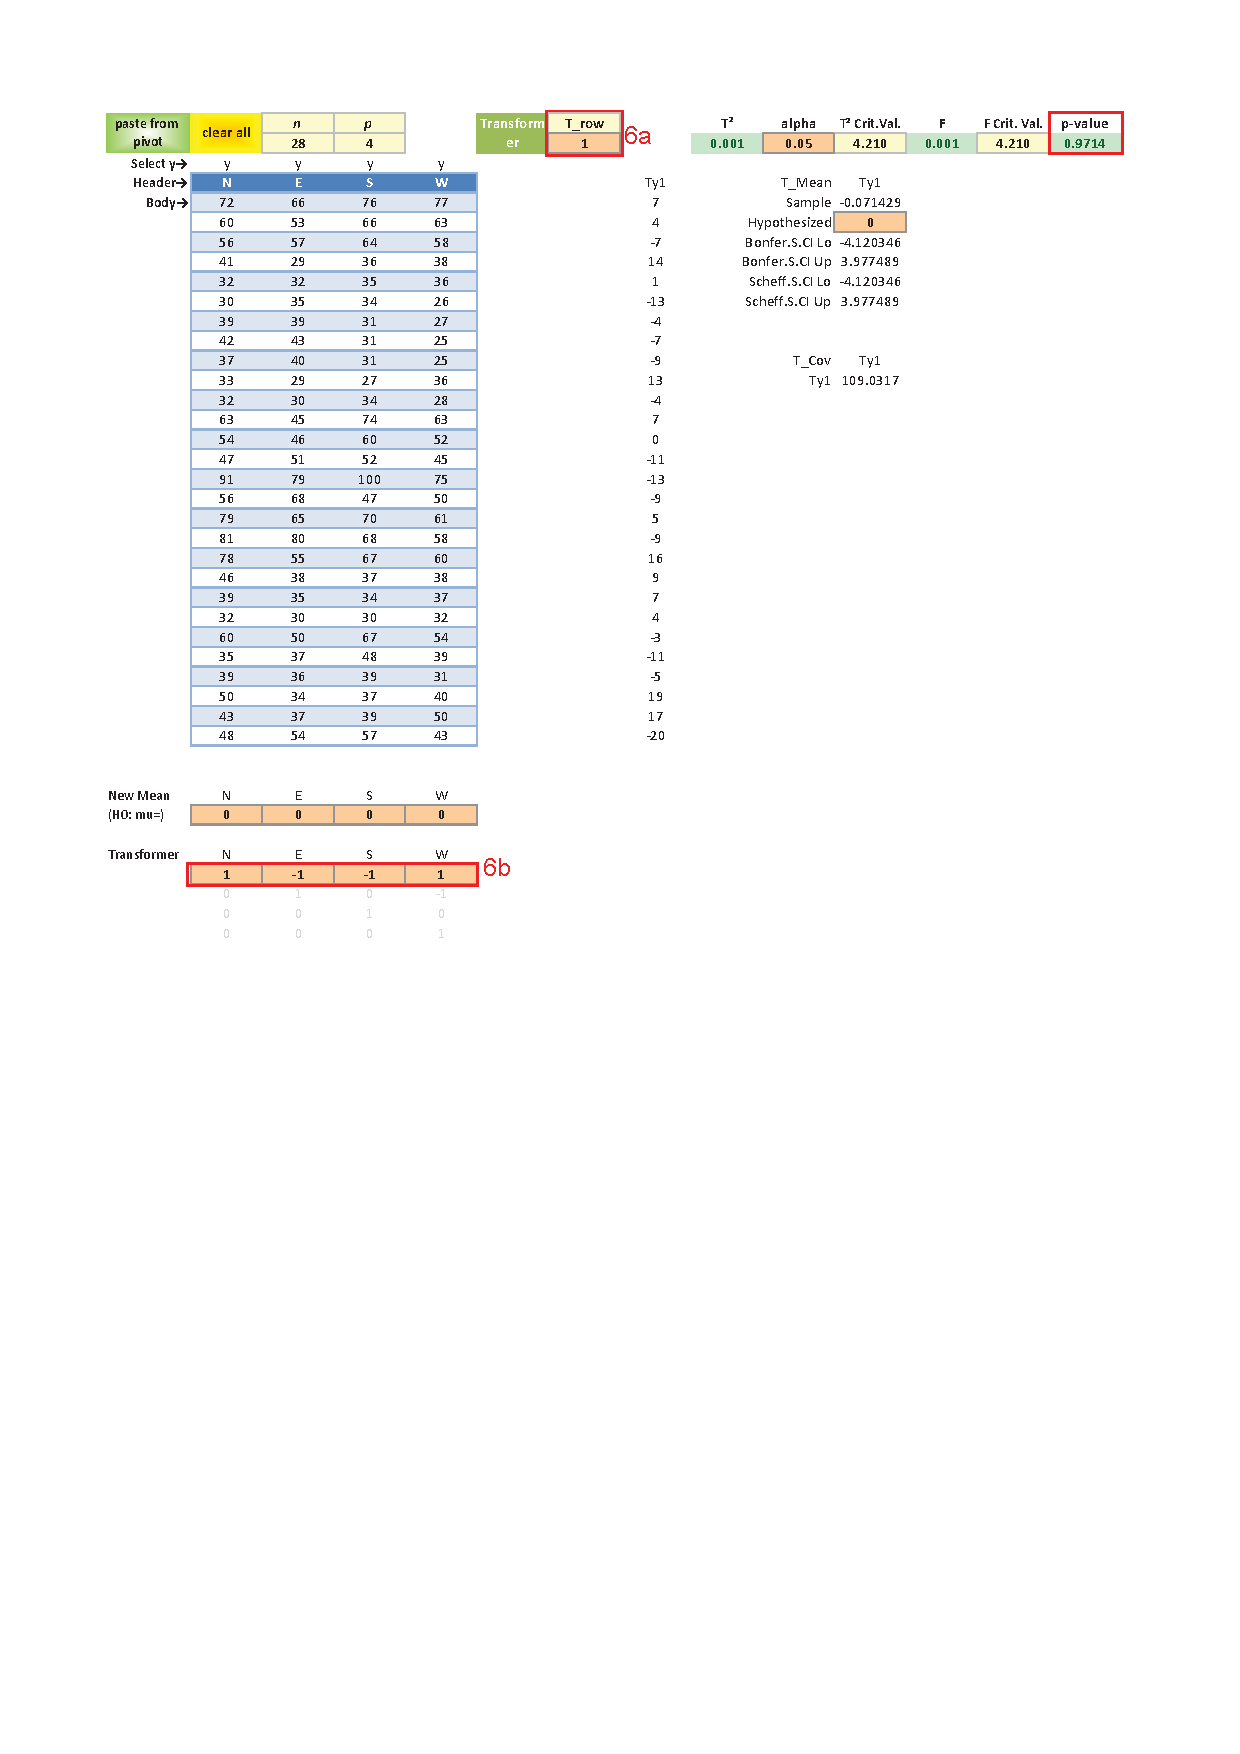
\includegraphics[width=\linewidth,keepaspectratio=true]{img/TsquareSheetOutput4_markup}
                \vspace{-20pt}\centering\protect\caption{Tsquare sheet: Testing $N-S=E-W$.}\label{fig:TsquareSheetOutput4}
        \end{figure}
        
        
        Note because $(1,-1,-1,1) = (1,0,-1,0) - (0,1,0,-1)$, therefore we cannot test all three hypotheses in one transformation as that would create a singular covariance matrix for the transformed data and then no $T^2$ statistic could be constructed.
        
        
        
        
        \subsection[egPCA]{Principal Component Analysis}
        Men's track data.
        \begin{enumerate}
          \item Locate the dataset under name ``Men" on the \shtData sheet using dropdown menu at cell \texttt{Data!A2} and copy it to clipboard
          \begin{center}
            \vspace{-20pt}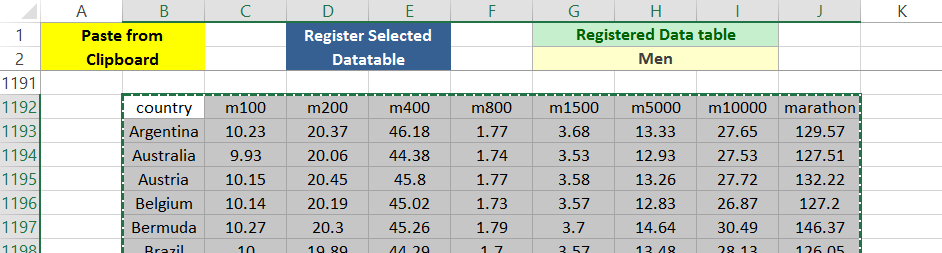
\includegraphics[height=200pt, keepaspectratio=true]{DataSheet_Men_png}
          \end{center}
          \item Activate the \shtPivot sheet and directly double-click the top-left green cell \texttt{Pivot!A1} to make a copy of the dataset and equip it with the Excel table format.
          \item Activate the \shtPCA sheet and directly double-click the top-left green cell \texttt{PCA!A1} to copy the data over.
          \begin{center}
            \vspace{-20pt}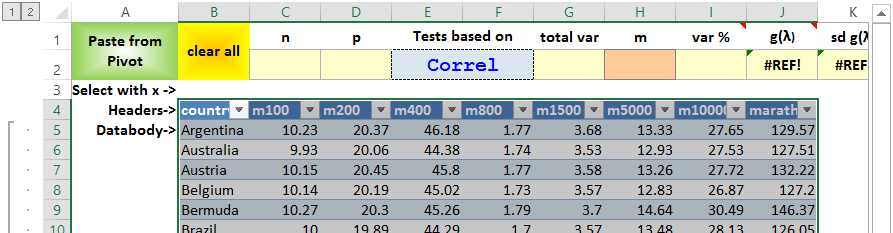
\includegraphics[width=\linewidth, keepaspectratio=true]{PCASheetAfterPaste_png}
          \end{center}
          \item Perform the following 3 steps exactly: Select cells \texttt{PCA!C3:J3} | press \texttt{x} on the keyboard | Windows user: press \texttt{ctrl} + \texttt{Enter} on the keyboard; Mac user: Press \texttt{command} + \texttt{Enter}. By doing these steps, you have entered 8 ``x"s simultaneously.
        \end{enumerate}
        The \shtPCA sheet should now appear as
        \begin{center}
          \vspace{-20pt}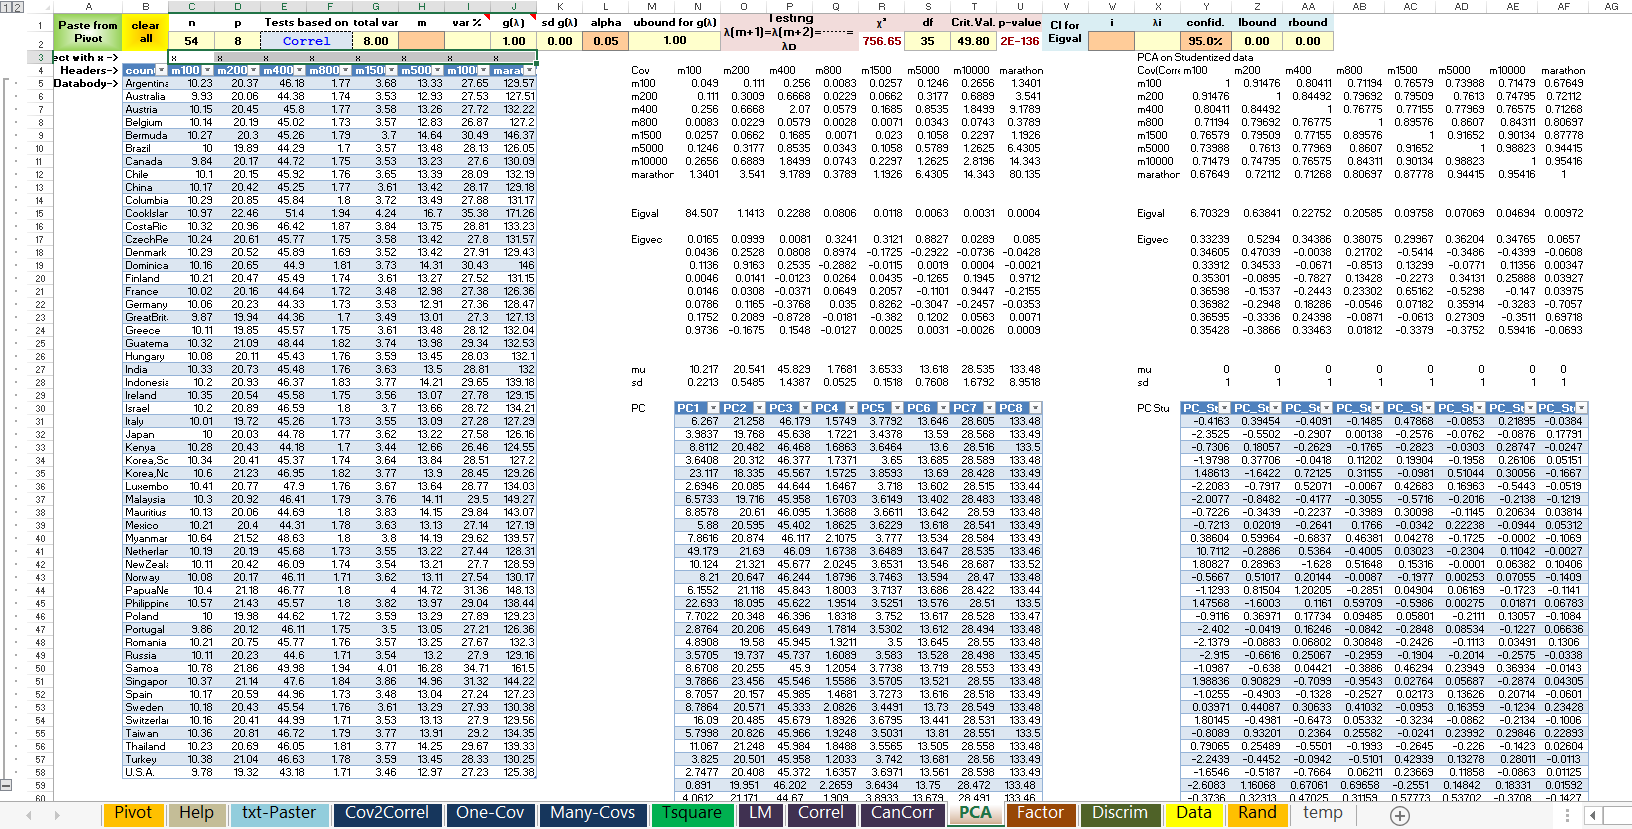
\includegraphics[width=\linewidth,keepaspectratio=true]{PCASheetOutput_png}
        \end{center}
        The main purpose of principal component analysis is dimension reduction and, if one assumes multivariate normality of data, de-correlation as a side effect. The \shtPCA sheet implements principal component analysis with the multivariate normality assumption. Under the assumption, PCA amounts to eigen-decomposition of the covariance matrix because the eigenvectors give the principal axes of the elliptic contour of the data. The longest principal axis is the linear direction on which the data projects to maximum variance. The second longest principal axis gives the next maximum-variance linear direction, and so on.
        The covariance matrix is always real-symmetric and have a set of orthogonal eigenvectors with positive eigenvalues. The eigenvalues have the interpretation as the variance of the multivariate data along the corresponding eigenvector direction.
        There is a subjective decision to make about whether studentization of data is needed. PCA on studentized data is equivalent to eigen-decomposition of the correlation matrix. The main issue is whether one wants to retain variance ratios among the observed variables. This certainly depends on the context. Ratios among some original variables may have established interpretations and hence would be preferred to retain. In other cases, for example, one is preparing the independent variables going into the right-hand side of a regression formula, one might want to studentize the data as the regression coefficients can recover such ratio. In middle cases, a properly estimated convex combination between the two matrices might be considered.
        Following are some further details regarding implementation.
        \begin{enumerate}
          \item PCA on correlation matrix do not add back the mean vector because if we do that we must also multiply back the s.d. But we don't want to do that because the s.d. is now unity for studentized data. This reflects that PCA on correlation matrix focuses on the angular difference between coordinates and ignores the radial differences.
          \item PCA on covariance matrix may add back the mean vector. The PCA on multivariate normal sample is essentially doing a rotation of the sample space about the mean vector, not the origin. To carry out that rotation via a rotation matrix, we need to first remove the mean before applying the rotation matrix formed by the eigenvectors, and may or may not add the mean vector back.
          \item PCA is essentially a data orthogonalization routine and does not model the mean vector. It can be used to orthogonalize the covariates for regression if prediction is the main goal and interpretation of the new covariates' meaning is not a concern. A more important purpose is dimension reduction. Those eigenvectors with a tiny eigenvalue indicate insufficient information in those trailing dimensions and hence could be removed to avoid over-fitting.
        \end{enumerate}
        Note that the original definition of PCA is to be a method seeking the linear directions on which data projects with maximum variance. With this definition, it is not restricted to multivariate normal data but is applicable under any sampling assumption by proper techniques. Nonetheless, if we can assume multivariate normality, the computation becomes much easier.
        
        
        
        
        
        \subsection[egCCA]{Correlation Analysis with Excel Tool}
        We use Salespeople Data to demonstrate canonical correlation analysis following \cite{anderson2003introMVA3e} The raw data can be located with name ``Salespeople" on the \shtData sheet 
            \begin{center}
              
\includegraphics[height=200pt, keepaspectratio=true]{img/DataSheet_Salespeople}
              \vspace{-20pt}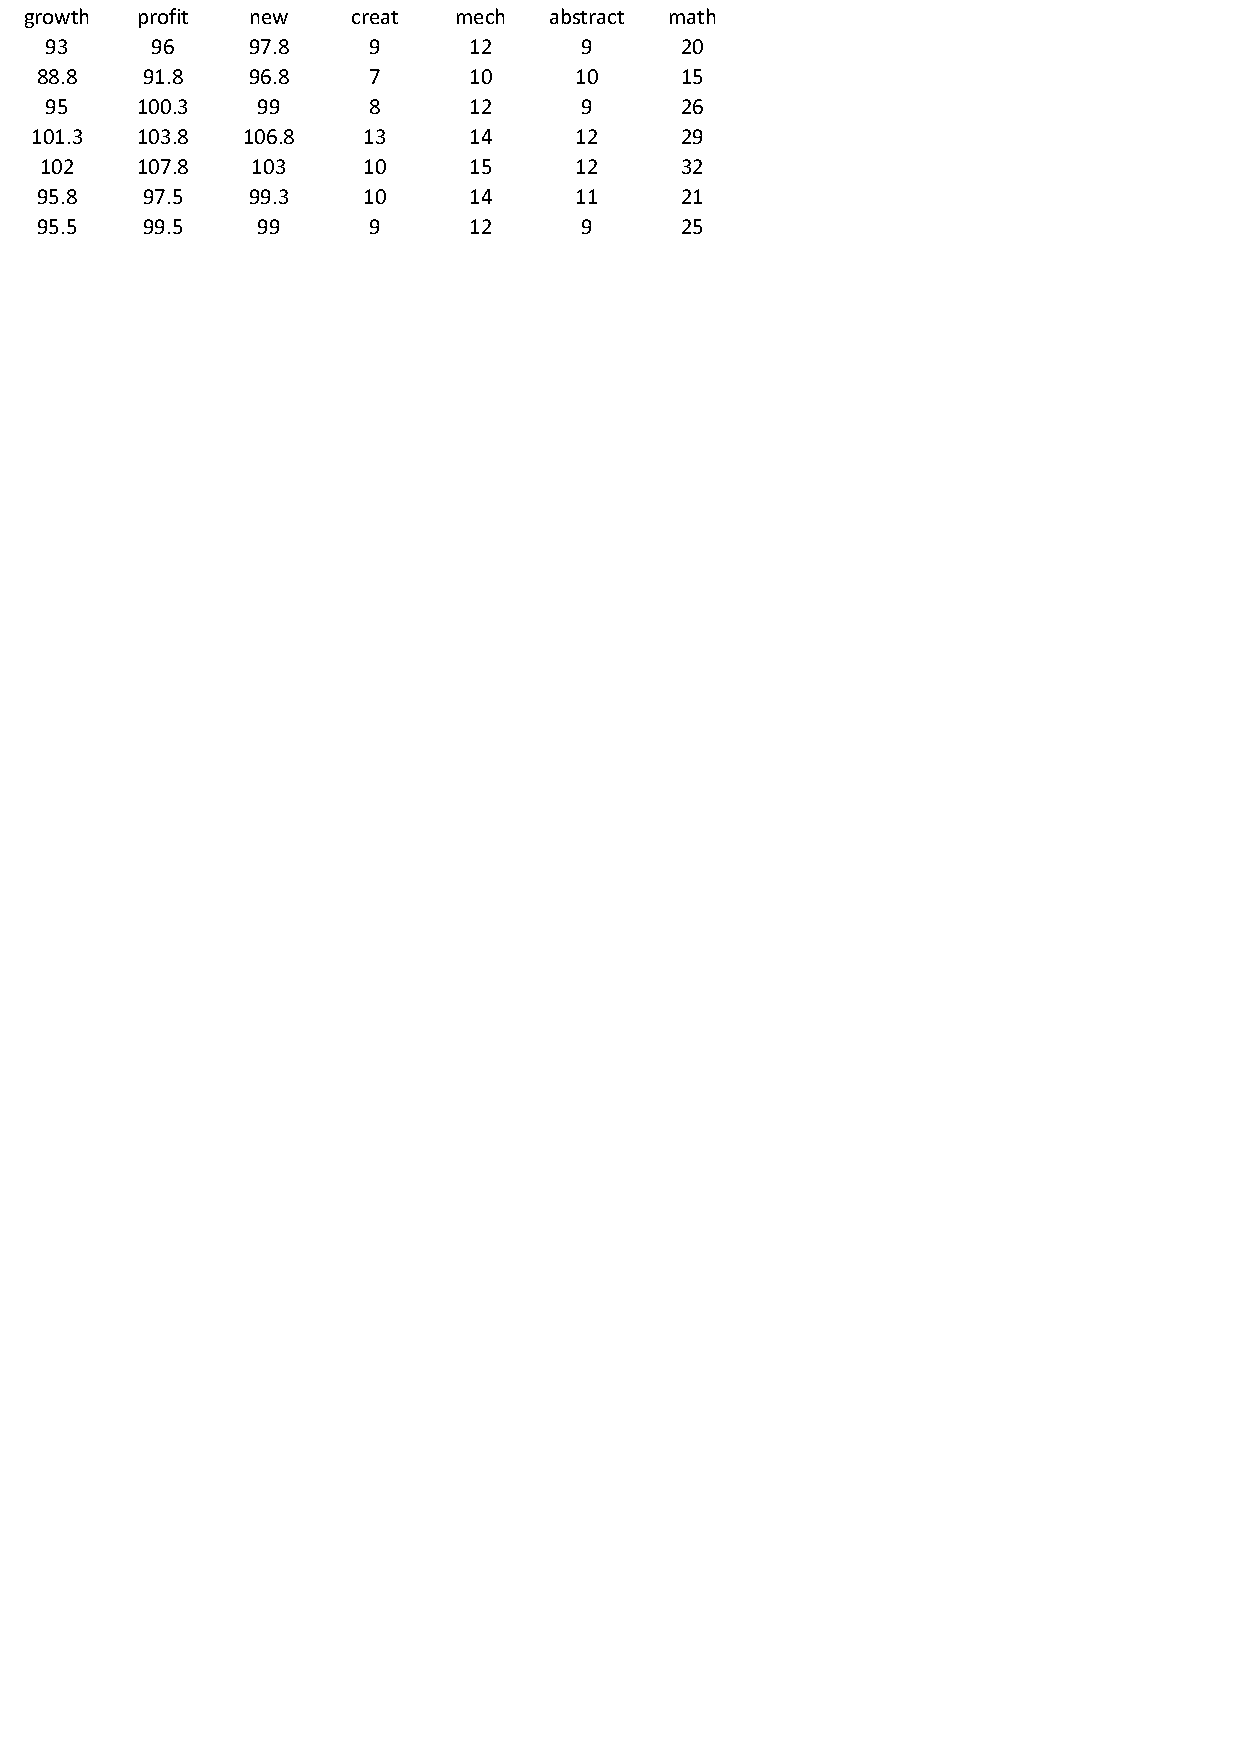
\includegraphics[height=200pt, keepaspectratio=true]{img/DataSheet_Salespeople2}
            \end{center}
        As before, the raw data should be copied first to the \shtPivot sheet, and then brought to the \shtCanCorr sheet using the green paste-from-pivot double-click button. We will investigate the correlation structure between the 3 performance variables and the 4 skill variables. To indicate grouping, we put a letter \texttt{v} ahead each column of a performance variable and a letter \texttt{w} ahead each column of a skill variable. The \shtCanCorr sheet should now appear as
        \begin{center}
          \vspace{-20pt}
\includegraphics[width=\linewidth,keepaspectratio=true]{img/CanCorrSheetOutput}
        \end{center}
        The overall idea of Canonical Correlation \cite{hotelling1936relations} Analysis is to construct a scalar ``correlation measure" $r$ to describe linear association between two vectors of multivariate random variables $\textbf{v}\in\mathbb{R}^p$ and $\textbf{w}\in\mathbb{R}^q$. The scalar is constructed by finding in each space a unit directional vector such that the usual unsigned correlation (geometrically the cosine of the angle) between the two directional vectors are maximal. The derivation of the pair of optimal directional vectors happens to become eigenvalue problems for two positive semi-definite matrices. The two matrices happen to share the a same set of non-zero eigenvalues and the largest eigenvalue is the square ``correlation" measure being sought. Moreover, the eigenvectors corresponding to the largest eigenvalue for each matrix is the unit vector in the respective space.
        \[\begin{gathered}
        r^2\textbf{v}  = \textbf{S}_{vv}^{ - 1}{\textbf{S}_{vw}}\textbf{S}_{ww}^{ - 1}{\textbf{S}_{wv}}\textbf{v}  \hfill \\
        r^2\textbf{w} = \textbf{S}_{ww}^{ - 1}{\textbf{S}_{wv}}\textbf{S}_{vv}^{ - 1}{\textbf{S}_{vw}}\textbf{w}  \hfill \\ 
        \end{gathered} \]
        \begin{center}
          \vspace{-20pt}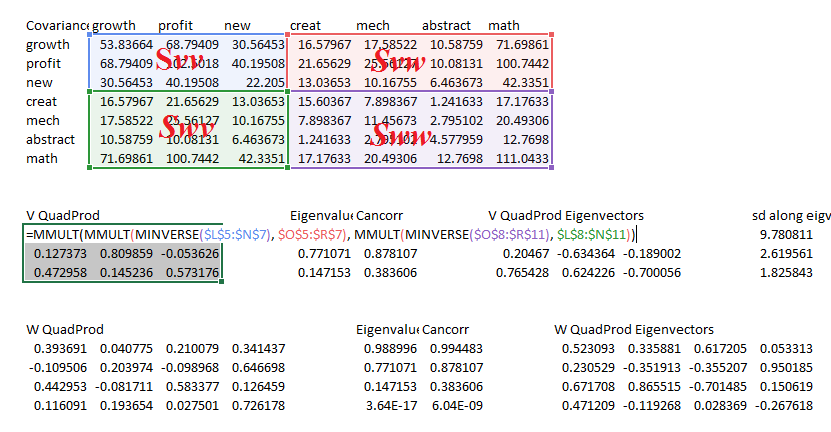
\includegraphics[width=\linewidth, keepaspectratio=true]{CanCorrSheetExplain_png}
        \end{center}
        For the second-largest eigenvalue, it is the squared canonical correlation between the spaces $\alpha^\bot\subset\mathbb{R}^{p-1}$ and $\beta^\bot\subset\mathbb{R}^{q-1}$, the orthogonal complement spaces of the two directional vectors, and recursively so doing for the other smaller non-zero eigenvalues. Note that the ``QuadProd" matrices are real symmetric, this means that the eigenvectors are perpendicular to each other. Together with the ``maximal correlation" property, the eigenvectors can be used to re-coordinate the data columns, as done in range starting at cell \texttt{CanCorr!AG4} and \texttt{CanCorr!AP4}. Figure \ref{fig:CanCorrSheetCanCorrVariates} shows first a few rows of re-coordinated data.
        \begin{figure}[!tbh]
          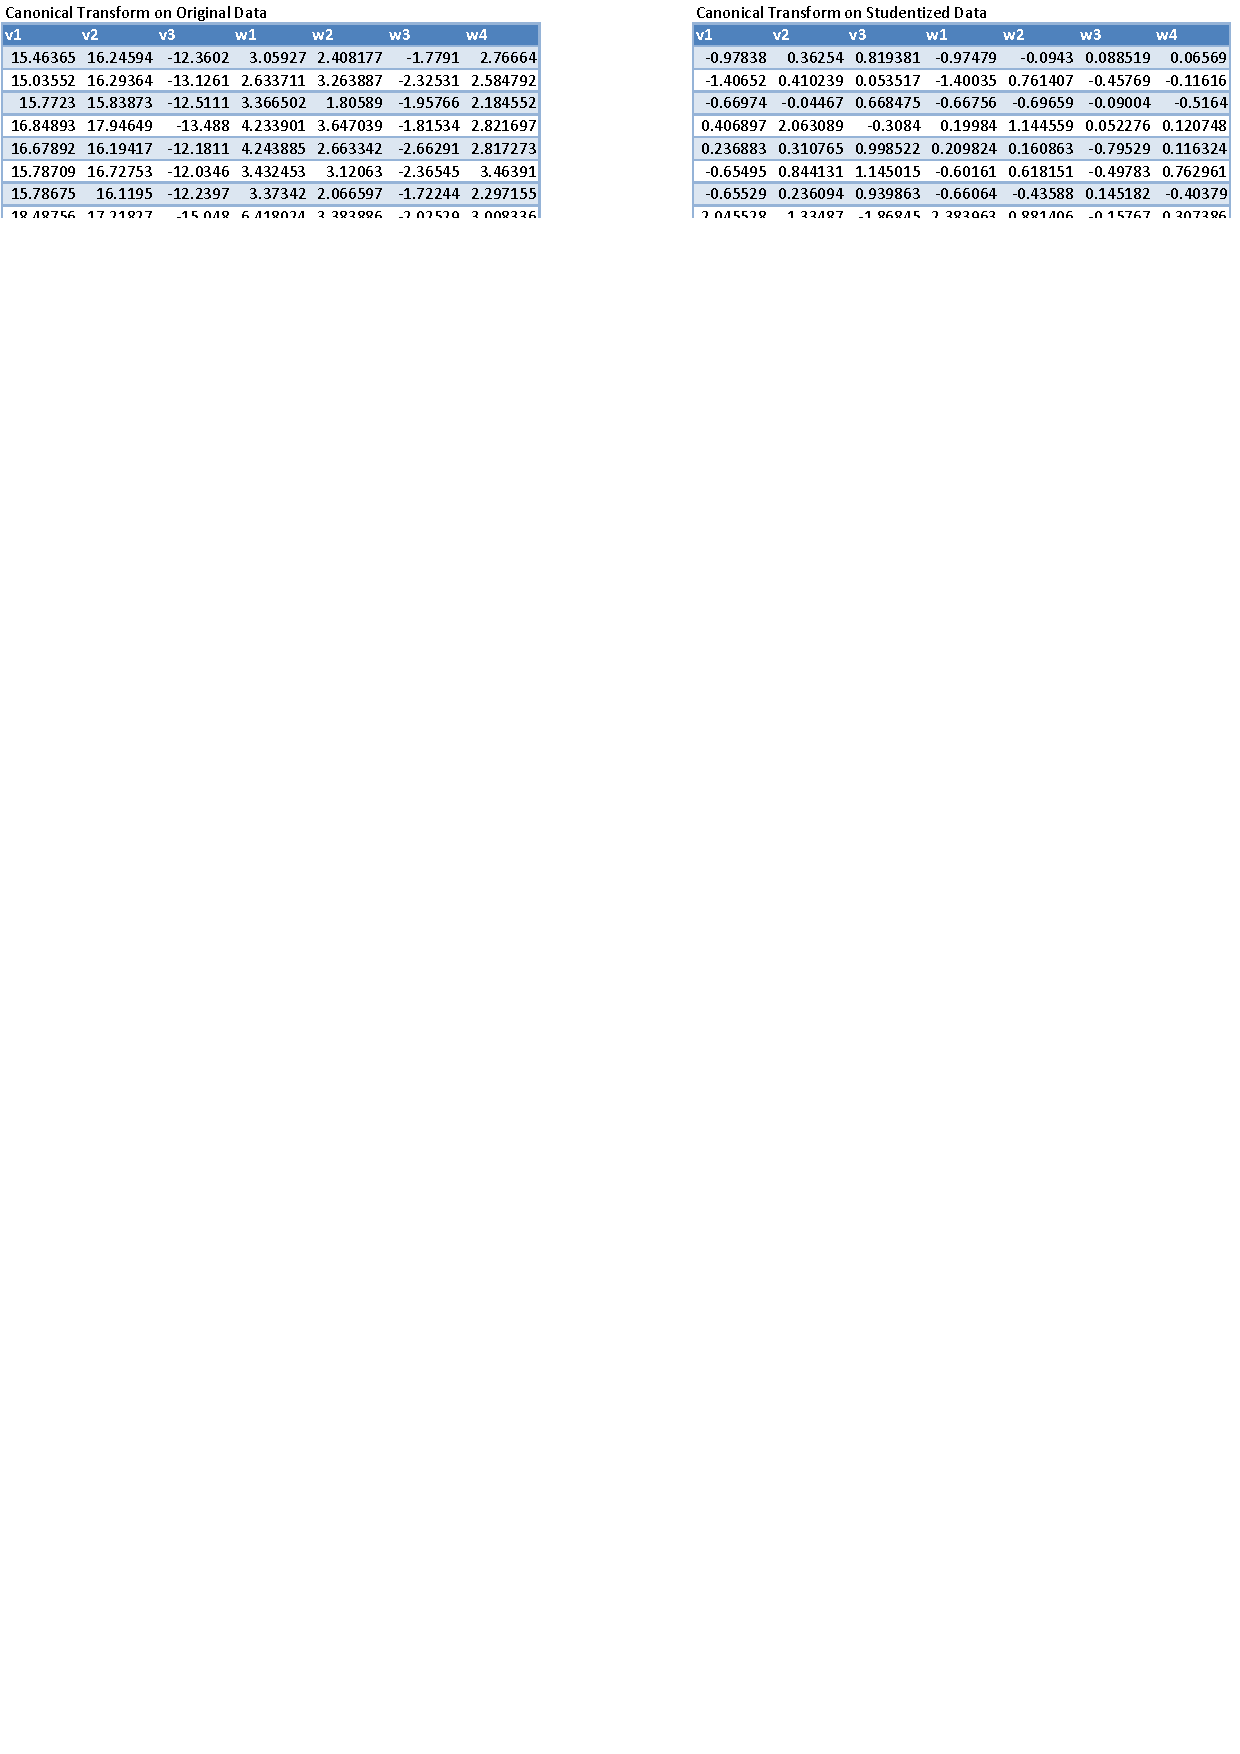
\includegraphics[width=\linewidth, keepaspectratio=true]{img/CanCorrSheetCanCorrVariates}
          \vspace{-20pt}\centering{}\protect\caption{Canonical Variates}\label{fig:CanCorrSheetCanCorrVariates}
        \end{figure}
        The full correlation matrix including the original dataset and the constructed canonical variates is displayed in range starting at cell \texttt{CanCorr!AY3}.
        \begin{center}
          \vspace{-20pt}
\includegraphics[width=\linewidth, keepaspectratio=true]{img/CanCorrSheetFullCorrel}
        \end{center}
        The fact that each V-canonical variate only respond to one of the W-canonical variates means that if we run a regression of all V's on all W's, then we know it is merely a bunch of 1-to-1 simple linear regression performed together.
        
        Finally, the first two rows implements some hypothesis tests to determine how many canonical variates should be retained if dimension reduction is a concern.
        \begin{center}
          \vspace{-20pt}
\includegraphics[width=\linewidth, keepaspectratio=true]{img/CanCorrSheetHypothesisTests}
        \end{center}
        
        
        
        
        
        \subsection[egFactor]{Factor Analysis with Excel Tool}
        When all observed variable are used and the residuals are still not spherical, one ponders over the existence of latent factors. The factor model is formulated as
        $$y  - \mu = \Lambda F + \varepsilon$$
        where $F$ is a multivariate normal vector that can be required to satisfy 
        $${\mathop{\rm var}} \left( F \right) = I$$
        and $\varepsilon$ is the new residual that is hopefully more spherical than before. The coefficient matrix $\Lambda$ is called the factor loadings. Both $F$ and $\Lambda$ will need to be estimated. A further simplifying assumption makes $\Lambda$ constant so that
        $${\mathop{\rm var}} \left( {\Lambda F} \right) = \Lambda {\Lambda ^\intercal}$$
        hence
        $${\mathop{\rm var}} (y - \mu ) = \Lambda {\Lambda ^\intercal} + {\mathop{\rm var}} \left( \varepsilon  \right).$$
        This suggests expanding the real-symmetric left-hand side by eigen-decomposition
        \[{\mathop{\rm var}} (y - \mu ) = {\lambda _1}{v_1}v_1^\intercal + {\lambda _2}{v_2}v_2^\intercal +  \cdots  + {\lambda _p}{v_p}v_p^\intercal\]
        and estimating $\Lambda {\Lambda ^\intercal}$ by first $m$ terms of this summation. This is the method implemented in the Excel tool.
        After $\Lambda$, the factor loadings matrix, is estimated, one then proceed to estimate $F$ by, for example, least square. In the Excel tool, we follow \cite{anderson2003introMVA3e} to implement the weighted least square method of \cite{bartlett1938}
        \[\hat F = {\left( {{\Lambda ^\intercal}{\Psi ^{ - 1}}\Lambda } \right)^{ - 1}}{\Lambda ^\intercal}{\Psi ^{ - 1}}z\]
        and the conditional expectation method of \cite{Thomson1951}
        \[\hat F = {\Lambda ^\intercal}{\left( {\Lambda {\Lambda ^\intercal} + \Psi } \right)^{ - 1}}z = {\left( {I + {\Lambda ^\intercal}\Psi \Lambda } \right)^{ - 1}}{\Lambda ^\intercal}{\Psi ^{ - 1}}z.\]
        In the following example, we analyze the olympic88 men decathlon data using factor analysis. The dataset doesn't contain any covariants, making it suitable to demonstrate the latent factor approach.
        
        1988 Summer Olympics Men's Decathlon data. 
        %Background: \texttt{https://en.wikipedia.org/wiki/Athletics\_at\_the\_1988_Summer_Olympics_\%E2\%80\%93_Men's_decathlon}
        \begin{enumerate}
          \item Locate the dataset under name ``Olympic88" on the \shtData sheet using dropdown menu at cell \texttt{Data!RegisteredList} and copy it to clipboard.
          \begin{center}
            
\includegraphics[height=200pt, keepaspectratio=true]{img/DataSheet_Olympic88_Selector}\\
            \vspace{-20pt}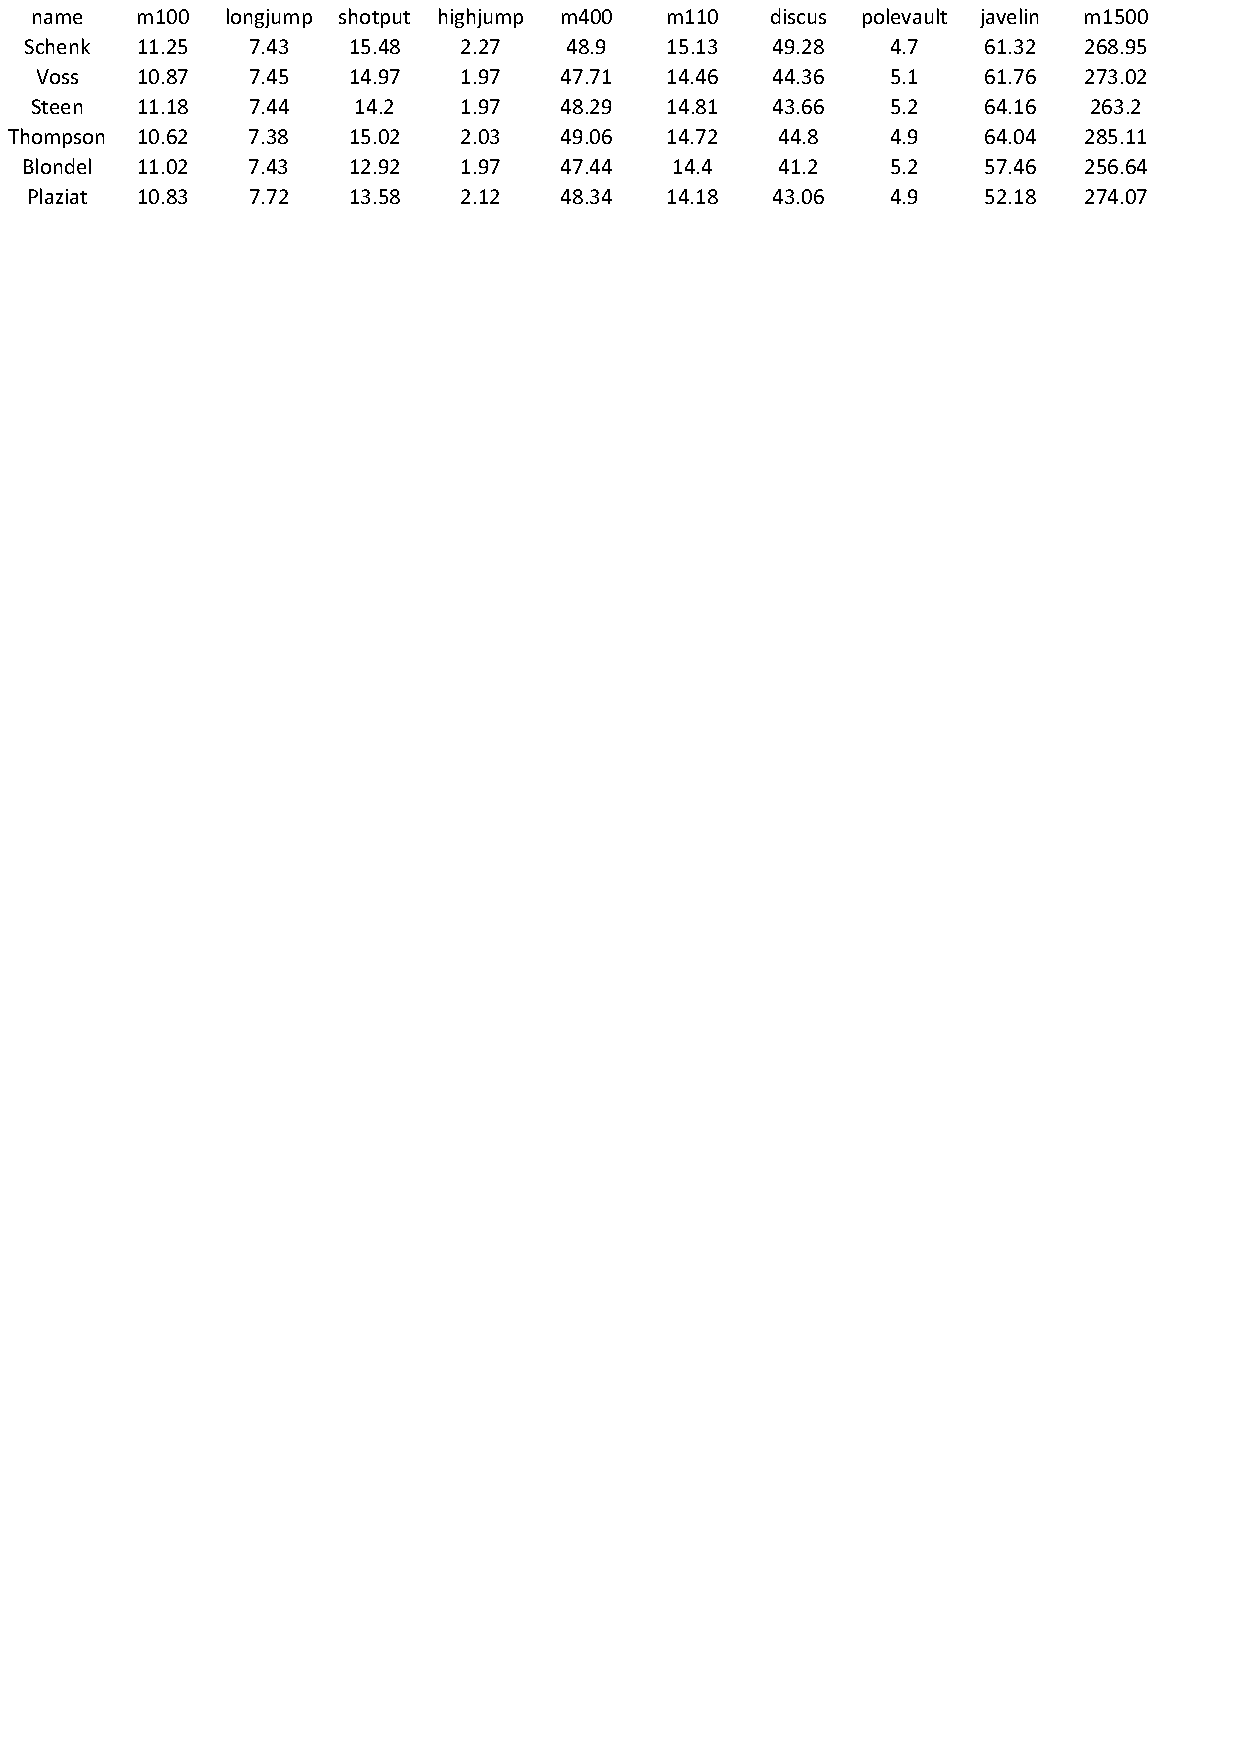
\includegraphics[height=200pt, keepaspectratio=true]{img/DataSheet_Olympic88_Data}
          \end{center}
          \item Activate the \shtPivot sheet and directly double-click the top-left green cell \texttt{Pivot!A1} to make a copy of the dataset and equip it with the Excel table format.
          \item Activate the \shtFactor sheet and directly double-click the top-left green cell \texttt{Factor!A1} to copy the data over.
          \begin{center}
            \vspace{-20pt}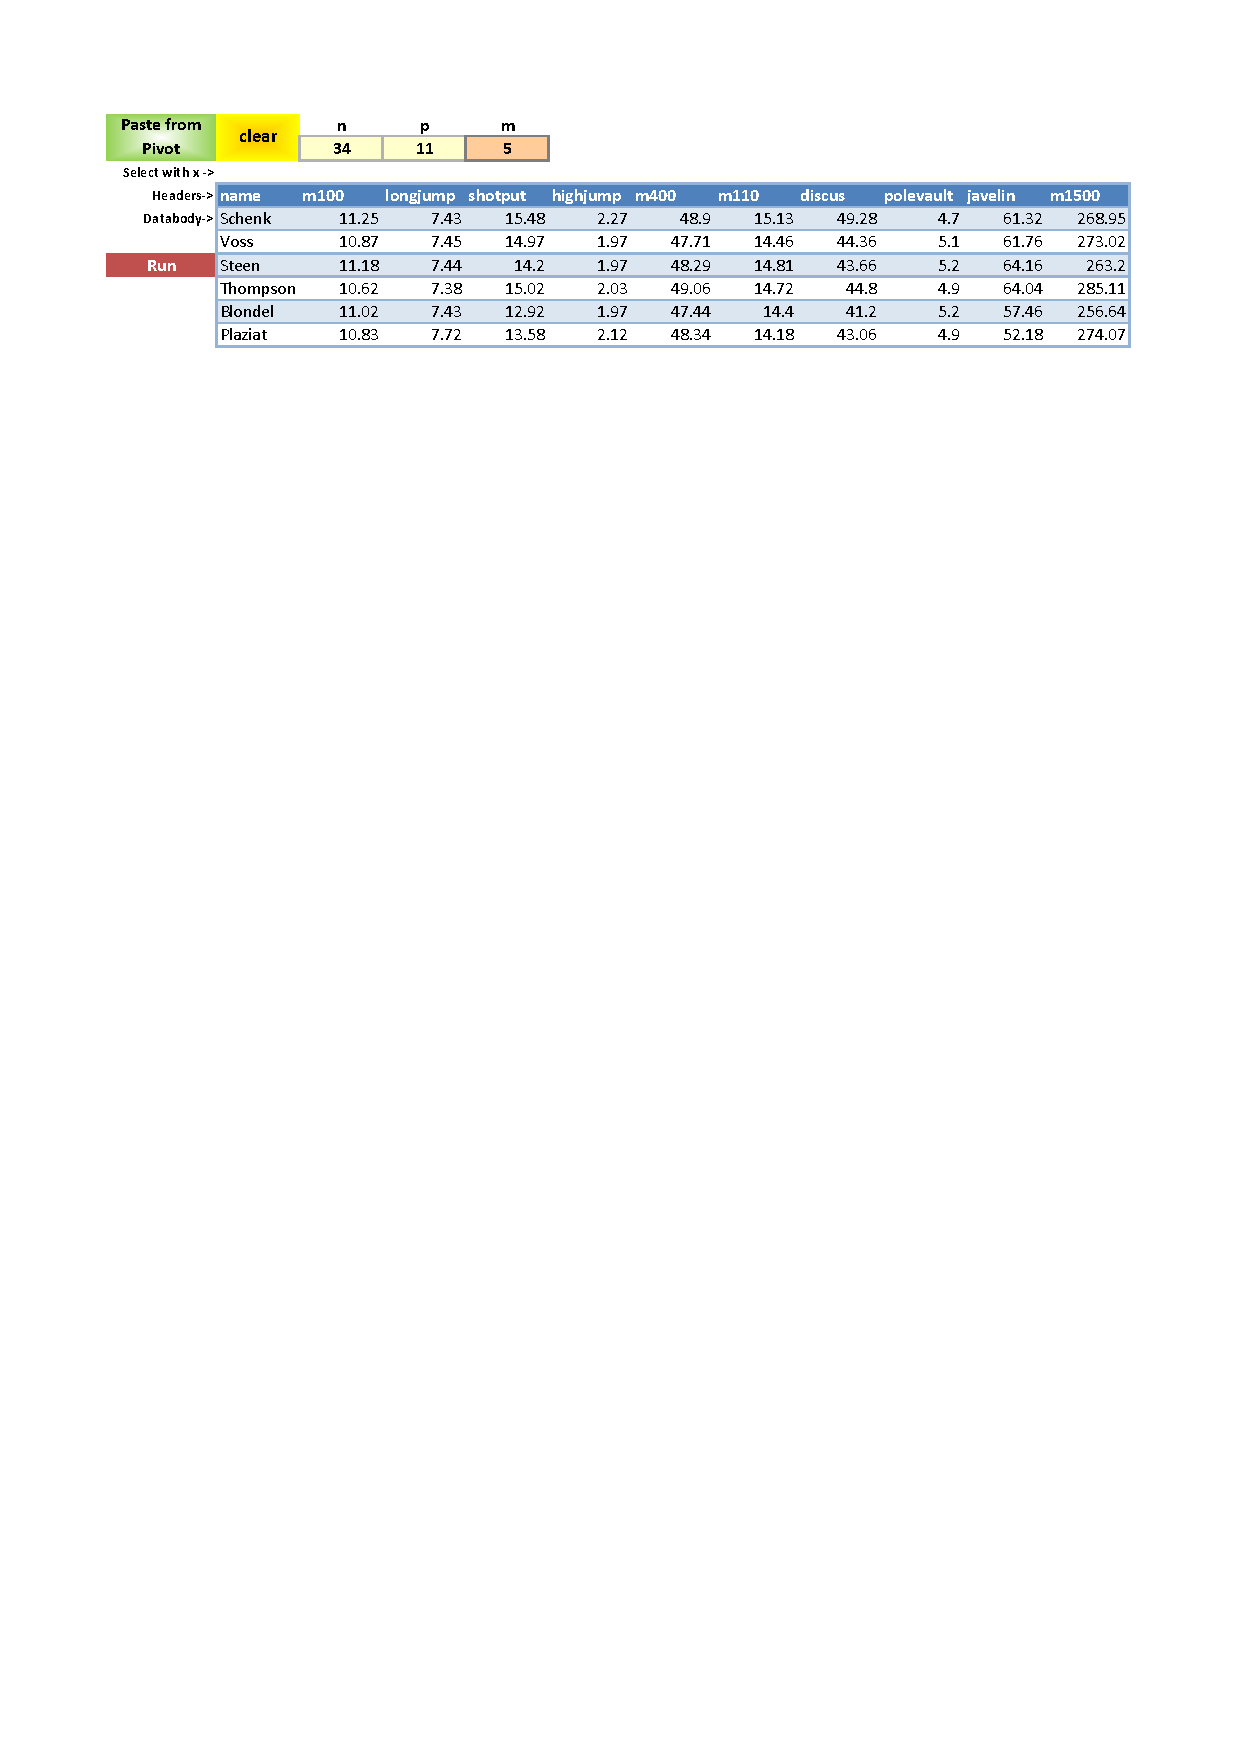
\includegraphics[width=\linewidth, keepaspectratio=true]{img/FactorSheetAfterPaste}
          \end{center}
          \item Perform the following 3 steps exactly: Select cells \texttt{Factor!C3:L3} | press \texttt{x} on the keyboard | Windows user: press \texttt{ctrl} + \texttt{Enter} on the keyboard; Mac user: Press \texttt{command} + \texttt{Enter}. By doing these steps, you have entered 10 ``x"s simultaneously.
        \end{enumerate}
        The \shtFactor sheet should now appear as Figure \ref*{fig:FactorSheetOutput_markup}. The heat-mapped regions on the right are 6 factor scores from different scoring methods and whether the input data has been studentized.
        \begin{figure}[!tbh]
          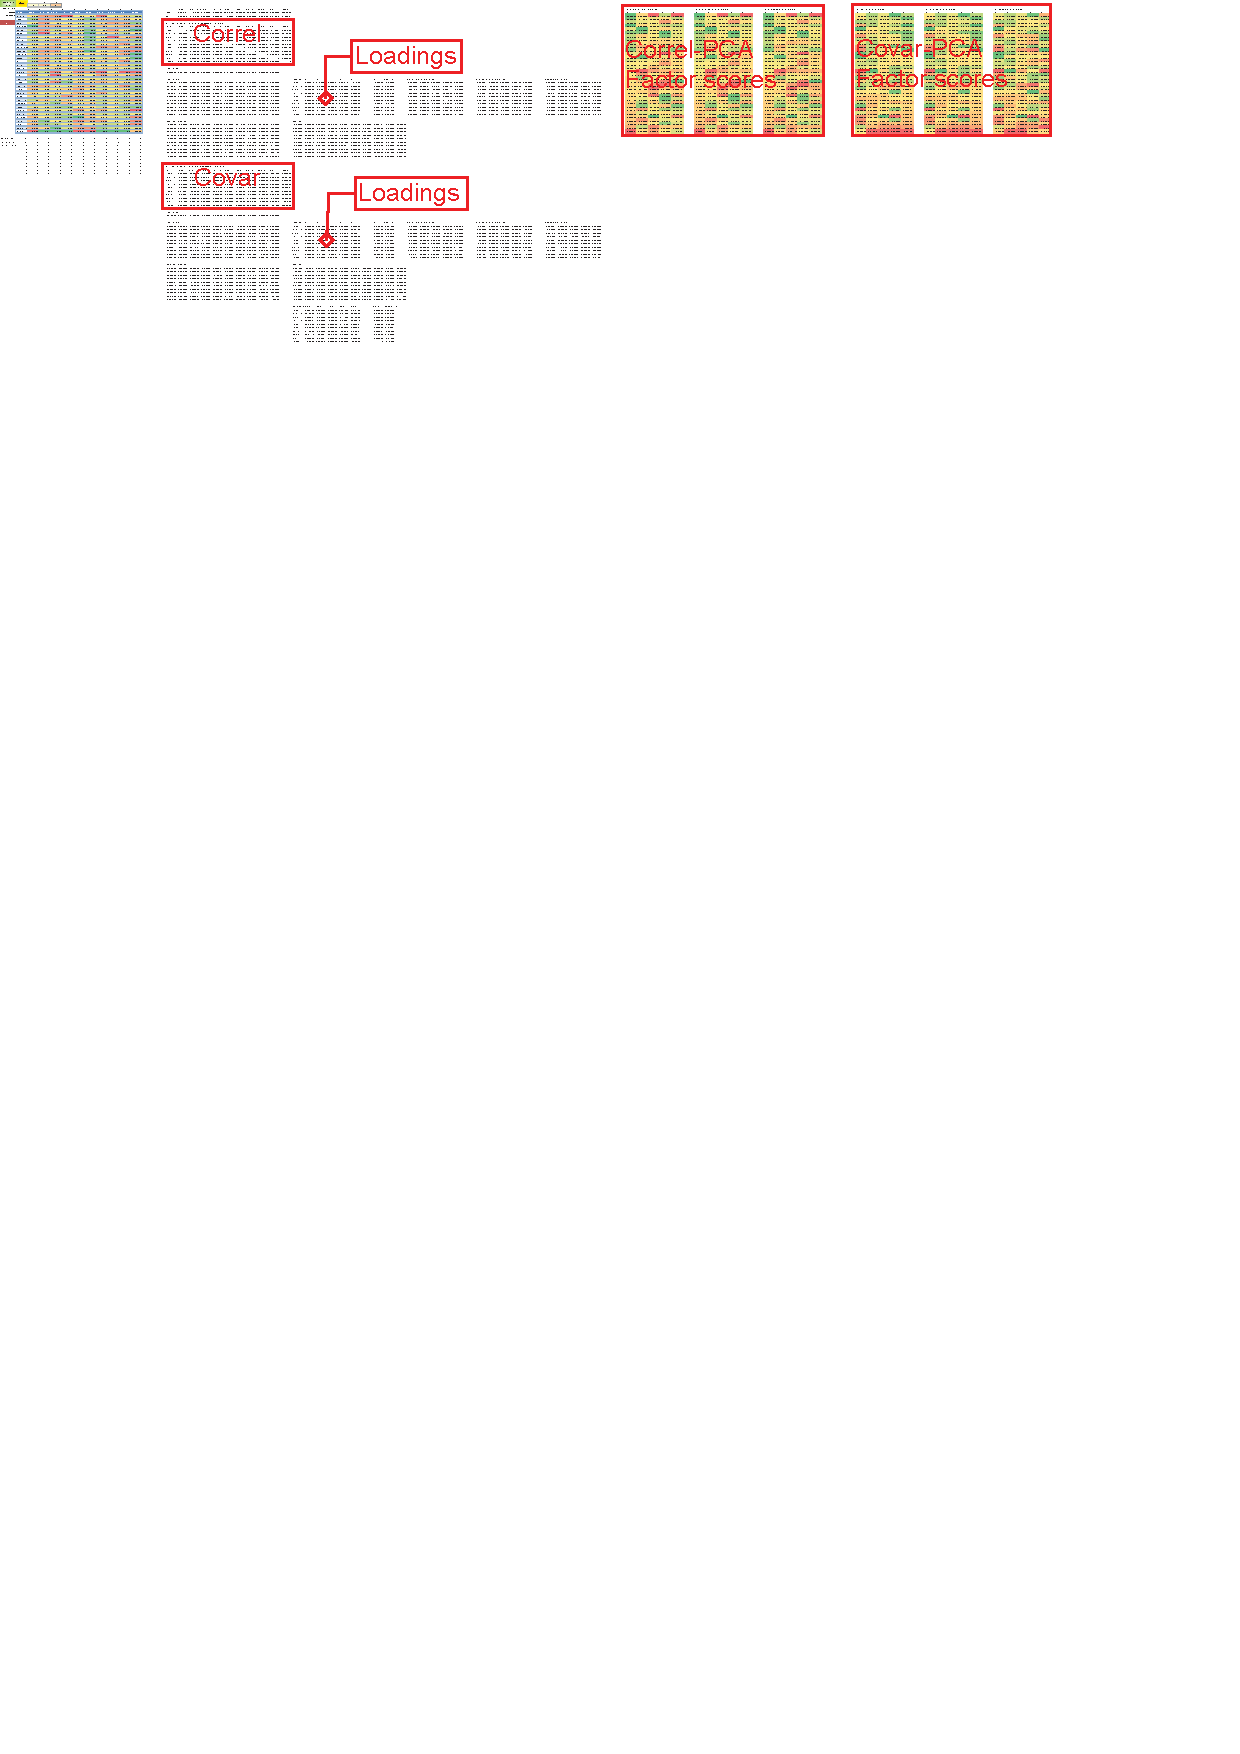
\includegraphics[width=\linewidth,keepaspectratio=true]{img/FactorSheetOutput_markup}
          \vspace{-20pt}\centering{}\protect\caption{Output from the Factor Analysis sheet}\label{fig:FactorSheetOutput_markup}
        \end{figure}

        
        \section[data]{Storing Data}
        The data import/export of the tool is delegated to Excel's own data i/o utilities. The user can add a blank sheet to import the dataset from various original sources. Next, all datasets need to be transformed into the \textit{data frame} format, i.e., a matrix of data with column header texts. A row in the data frame is a multivariate sample vector jointly observed for all the variables and a column is a univariate sample observed repeatedly for a single variable. The number of rows in the data frame is the sample size. This format should be familiar to both \texttt{SAS} (sas7bdat) and \proglang{R} (data frame) users. 
        
        After importing and transforming into the data frame format, the dataset should be registered on the sheet \shtData and archived there for future usage. The sheet \shtData can be navigated via a dropdown menu near cell \texttt{Data!A2}, which lists all registered datasets. 
        
        A working copy of a dataset should be put on the \shtPivot sheet.
        
        Following is an example of generating multivariate normal random sample using the \shtRand sheet and then registering and storing it on the \shtData sheet. \\
        \begin{enumerate}
        \item Activate sheet \shtRand.
        \item Put 3000 to \texttt{Rand!C2} to specify the sample size.
        \item Enter the mean vector as a column vector right below cell \texttt{Rand!D1}: $[0,0,0]^\intercal$
        \item Enter the covariance matrix as a symmetric positive-definite matrix right below cell \texttt{Rand!E1} and extend to the right:  
        \[\left[ {\begin{array}{*{20}{c}}
        9&5&-5 \\ 
        5&8&0 \\ 
        -5&0&7 
        \end{array}} \right]\]
        \end{enumerate}
        Sheet \shtRand should now appear as
        \begin{center}
	        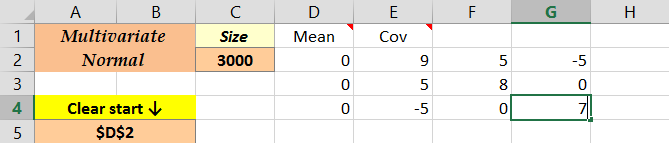
\includegraphics[height=64pt, keepaspectratio=true]{RandSheetAfterInput_png}
        \end{center}
        Now if you double-click on the cell \texttt{Rand!A7} (
\includegraphics[height=8pt, keepaspectratio=true]{RandSheet_GenerateButton_png}) some equation will be entered to the sheet by a \proglang{VBA} macro (\texttt{shtRand.generate}) triggered on the double-click event you just performed to the cell \texttt{Rand!A7}. The $3000\times 3$ range \texttt{Rand!E7:G3006} is also automatically selected so that you can directly press the scatter plot button to have a visual check as I am doing. Sheet \shtRand should now appear as
        \begin{center}
	        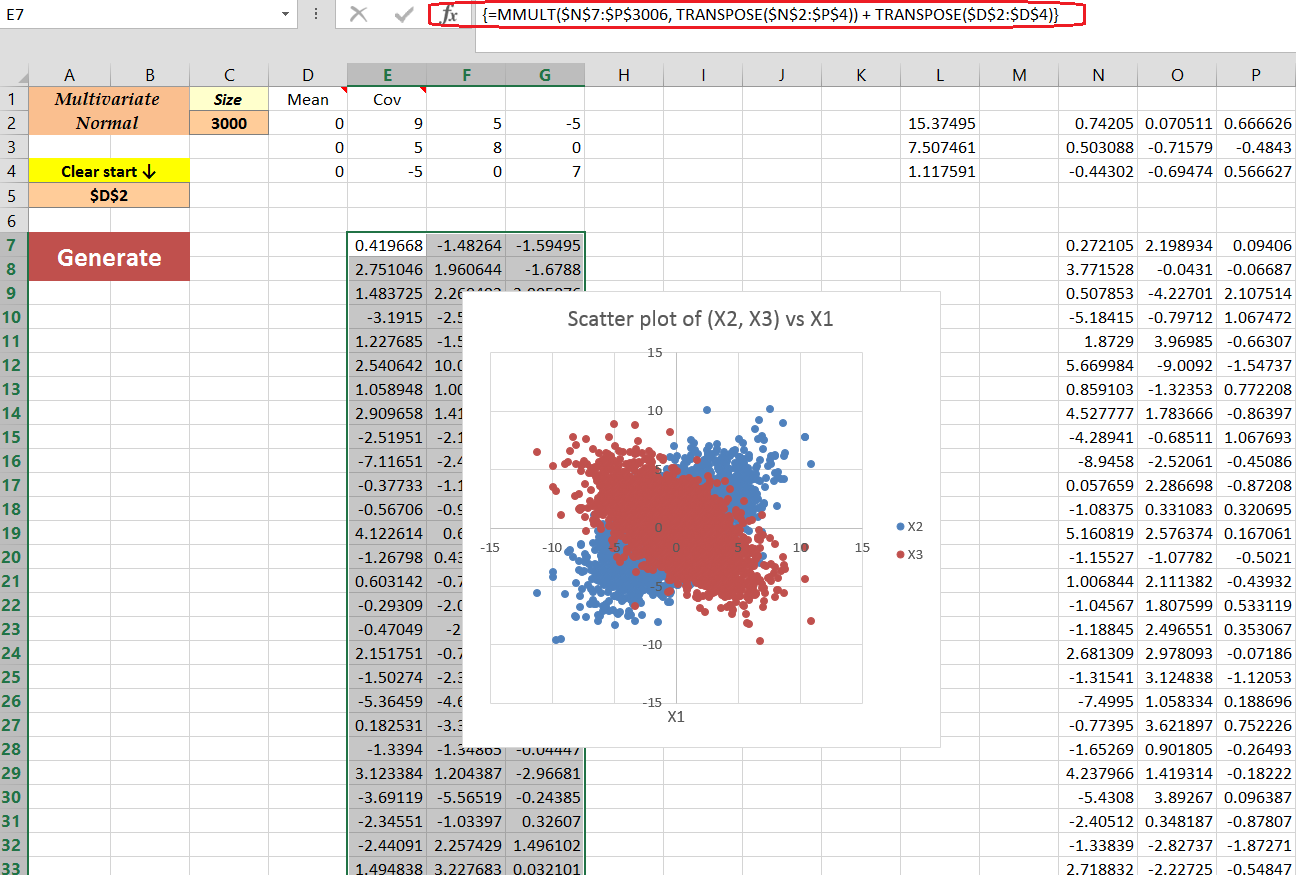
\includegraphics[width=\linewidth, keepaspectratio=true]{RandSheetOutput_png}
        \end{center}
        The quick visual check confirms that: (i) the mean location is near the origin, (ii) both data exhibits the elliptical contour consistent with the positive definite quadratic form embedded in the MVN density, and (iii) the positive correlation between X1 and X2 gives the $+45^\circ$ rotation of the blue sample while the negative correlation between X1 and X2 gives the $-45^\circ$ rotation of the red sample.
        
        A very important feature here is that the output is a function of the input and is connected to input via a formula chain. As a result, if the user changes the covariance input, then immediately the plot will update. This reveals the many upsides of using Excel to do mathematical modeling on small-to-medium sized data: it is a functional environment; it has a robust event system; it has a lot of productive utilities to operate the data; and it lets you monitor all variables at the same time. These are all conducive to (self-)teaching core multivariate statistics.
        
        Next we will register the generated random sample to the Data sheet. Note that the following step of storing and registering dataset on the tool is the same for any data as long as it is presented in the data frame format. One can leverage Excel's own utilities to prepare the raw data into the data frame format.
        \begin{enumerate}
        \item Add names to the 3 columns by typing into cells \texttt{Rand!E6:E8} ``X1", ``X2", ``X3". During the process the sample may be regenerated.
        \item Press ctrl+a on Windows or command+a on Mac to select the entire $3001\times 3$ data range \texttt{Rand!E6:G3006} (now with a header row)
        \item Press ctrl+c to copy to clipboard.
        \item Launch a simple text editor and paste the data there to make it plain text.
        \item Copy everything in the simple text editor to clipboard
        \item Activate sheet \shtData
        \item Double click on \texttt{Data!I1} (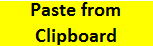
\includegraphics[height=16pt,keepaspectratio=true]{DataSheet_PasteFromClipboardButton_png}) to initiate pasting and registration of a new dataset
        \item Click \texttt{Yes} to confirm registration of this dataset to sheet \shtData
        \begin{center}
	        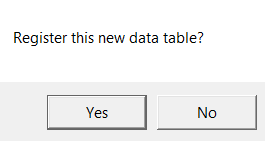
\includegraphics[height=80pt, keepaspectratio=true]{DataSheet_ConfirmRegister_png}
        \end{center}
        \item Enter "Random MVN 3000 x 3" to name the dataset being registered
        \begin{center}
	        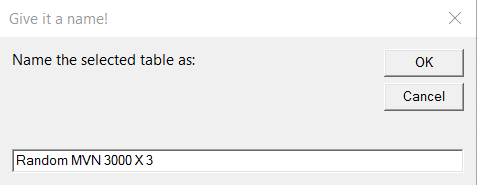
\includegraphics[height=80pt, keepaspectratio=true]{DataSheet_GiveDatasetName_png}
        \end{center}
        \item Roll out the dropdown menu at cell \texttt{Data!A2} and look for the newly registered dataset and select it. After select, the screen will auto-navigate to the dataset and select it.
        \begin{center}
	        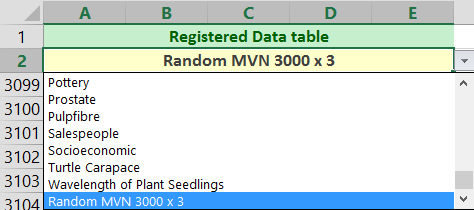
\includegraphics[height=120pt, keepaspectratio=true]{DataSheet_LocateDatasetViaMenu_png}
        \end{center}
        \item You can now press the keyboard shortcut to copy the selection to the system clipboard.
        \begin{center}
	        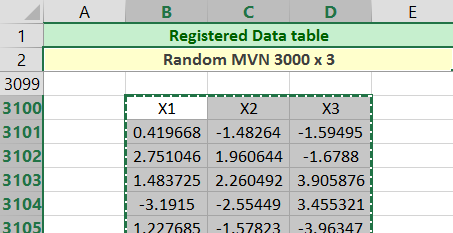
\includegraphics[height=136pt,keepaspectratio=true]{DataSheet_CopyDataset_png}
        \end{center}
        \item Once the data is on the clipboard, switch to the \shtPivot sheet and immediately double-click on the top-left green button
        \begin{center}
	        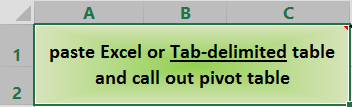
\includegraphics[height=42pt, keepaspectratio=true]{PivotPasteButton_png}
        \end{center}
        \item After double-click, the dataset will be pasted to the \shtPivot sheet as an Excel table and hence it enjoys all Excel table associated utilities such as filtering with complex conditions (\proglang{SQL} select in disguise), multi-column sort, pivot table (aggregation, a bit like \proglang{R} apply), and graphics. Depending on how you configure the pivot table, \shtPivot may now appear as
        \begin{center}
	        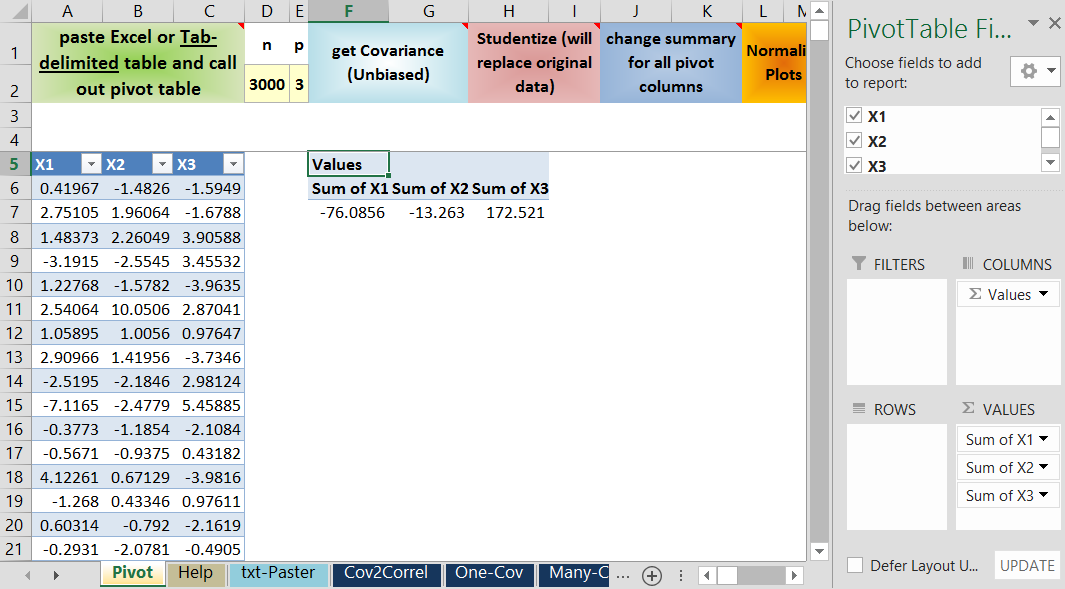
\includegraphics[width=\linewidth, keepaspectratio=true]{PivotSheetAfterPaste_png}
        \end{center}
        \item The cell \texttt{Pivot!J1} can help you change the aggregate function to one of \texttt{Sum}, \texttt{Count}, \texttt{Average}, \texttt{Max}, \texttt{Min}, \texttt{Product}, \texttt{Count numbers}, \texttt{stddev}, \texttt{stddevp}, \texttt{var}, and \texttt{varp}. This is a quick way to get the mean vector and the sd vector.
        \begin{center}
	        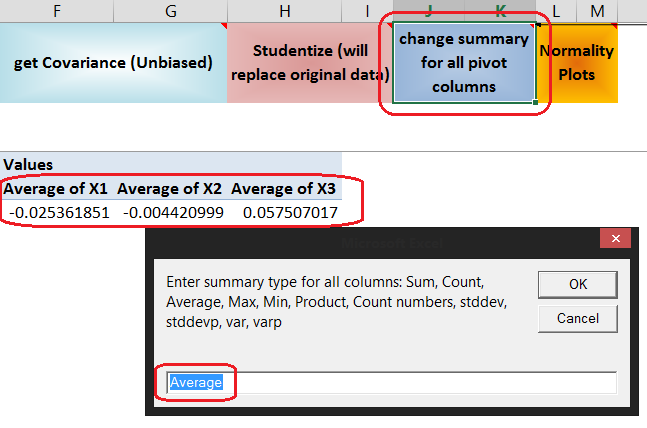
\includegraphics[width=\linewidth, keepaspectratio=true]{PivotSheetChangePivotAggregateFunc_png}
        \end{center}
        \item The orange button at cell \texttt{Pivot!L1} makes normal and $\chi^2$ QQ plots to help visually check marginal and joint normality. To do this, put an ``x" in cells \texttt{Pivot!A4:C4} above the column headers and then double click on the orange button. The \shtPivot sheet may now appear as
        \begin{center}
	        \includegraphics[width=\linewidth, keepaspectratio=true]{PivotSheetNormalityPlots_png}
        \end{center}
        The normal quantile-quantile plots are made by the \proglang{VBA} macro \texttt{NormalQQplot}. The chi-squared quantile-quantile plot for inspecting violation of joint normality is made by the macro \texttt{MahalanobisChisqQQplot}. The Mahalanobis distance is defined as \[D = \sqrt {{{\left( {\textbf{x} - \bar{\textbf{x}}} \right)}^ \intercal }{\textbf{S}^{ - 1}}\left( {\textbf{x} - \bar{\textbf{x}}} \right)} \]
        Its square has an asymptotic $\chi(p)$ distribution where $p$ is the number of variables ($p=3$ here).
        \end{enumerate}
        
        
        
        \section[software]{Discussion}
        The Excel tool is sheet-oriented. There four types of sheets: Data storage sheet (\shtData), Data simulation sheet (\shtRand), Data pre-process sheet (\shtPivot), and Method sheet (\shtLM, etc). The \shtPivot sheet contains the data in analysis-ready state. The method sheets all implement a paste-from-pivot button at the top-left corner to create its own copy of the analysis-ready data and then builds formula chains to arrive at results. All sheets can use built-in Excel functionalities as well as custom addin functions written in VBA, XLL(COM), or .NET(VSTO). The transparency of the computation together with Excel's own tools around formula building, tracing, and checking allows complex models to be understood quickly. It is also a good self-documentation of an implementation elsewhere such as R. We recommend all R implementation has an equivalent Excel Tool sheet. This will solve an important problem of getting one's implementation details understood, extended with confidence, and understood again.
        
        \bibliographystyle{jss}
        \bibliography{MasterBibliography}

\end{document}
